\documentclass[10pt, conference]{IEEEtran}
\usepackage{amsmath, amssymb, amsfonts}
\usepackage{graphicx}
\usepackage{booktabs}
\usepackage{tikz}
\usepackage{pgfplots}
\pgfplotsset{compat=1.18}

% --- Copyright Footer Code ---
\usepackage{fancyhdr}
\pagestyle{fancy}
\fancyhf{}
\renewcommand{\headrulewidth}{0pt}
\cfoot{\scriptsize \copyright~Author: Arpit Raj}

\fancypagestyle{plain}{
  \fancyhf{}
  \cfoot{\scriptsize \copyright~Author: Arpit Raj}
}
% -----------------------------

\title{Semantic Communication in 6G: ML/DL Implementation}

\author{\IEEEauthorblockN{Arpit Raj}
\IEEEauthorblockA{\textit{The LNM Institute of Information Technology (LNMIIT)}\\
Jaipur, India}
}

\begin{document}

\maketitle

\begin{abstract}
This research paper deals with next-gen semantic communication. As wireless networks approach the theoretical bounds of classical Shannon capacity, next-generation telecommunications (6G) must transition from exact bit-stream transmission to goal-oriented, semantic communication. This research presents an end-to-end software simulation of a semantic communication physical layer, demonstrating the inherent error resilience of natural language processing (NLP) embeddings over noisy wireless channels. Rather than mapping text to binary sequences, the proposed deterministic framework utilizes dense vector representations (e.g., Sentence-BERT) as joint source-channel coders. These high-dimensional mathematical representations of human intent are transmitted through a simulated Additive White Gaussian Noise (AWGN) channel under variable Signal-to-Noise Ratio (SNR) conditions. At the receiver, decoding is achieved not through classical binary error-correction, but via cosine similarity mapping against a localized vector knowledge base.
\end{abstract}

\section{\large \textbf{Conventional Communication}}
Conventional communication systems are built on Claude Shannon's information theory. In these architectures, the message is transmitted bit by bit. 

\subsection{\textbf{Source Encoder}}
The primary step in the communication flow is the source encoder. The goal here is to transform information into a source binary code while using as few bits as possible. A prominent method to achieve this and reduce redundancy is Huffman coding.

\section{\large \textbf{Huffman Coding Analysis}}

\subsection{\textbf{Fixed-Length Coding (Without Huffman)}}
To illustrate the necessity of Huffman coding, let us first consider a scenario without it, assuming every symbol uses a fixed length of 2 bits.

\begin{table}[h]
\centering
\caption{Fixed-Length Coding Probabilities}
\begin{tabular}{ccc}
\toprule
\textbf{Symbol} & \textbf{Probability} & \textbf{Code} \\
\midrule
A & 0.5   & 00 \\
B & 0.25  & 01 \\
C & 0.125 & 10 \\
D & 0.125 & 11 \\
\bottomrule
\end{tabular}
\end{table}

For a transmission of 100 symbols, the total number of bits required would be:
\begin{equation}
\text{Bits} = (50 \times 2) + (25 \times 2) + (12.5 \times 2) + (12.5 \times 2)
\end{equation}
\begin{equation}
\text{Total Bits} = 200 \text{ bits}
\end{equation}

\subsection{\textbf{Variable-Length Coding (With Huffman)}}
Huffman coding dictates that for more frequent symbols, the number of bits should be less. A fundamental rule for unique decoding is that no code starts with another complete code (prefix rule).

\begin{table}[h]
\centering
\caption{Huffman Coding Probabilities}
\begin{tabular}{ccc}
\toprule
\textbf{Symbol} & \textbf{Probability} & \textbf{Code} \\
\midrule
A & 0.5   & 0 \\
B & 0.25  & 10 \\
C & 0.125 & 110 \\
D & 0.125 & 111 \\
\bottomrule
\end{tabular}
\end{table}

For a 100-symbol message using Huffman coding, the total number of bits is calculated as:
\begin{equation}
\text{Bits} = (50 \times 1) + (25 \times 2) + (12.5 \times 3) + (12.5 \times 3)
\end{equation}
\begin{equation}
\text{Total Bits} = 175 \text{ bits}
\end{equation}
By utilizing this method, a total of \textbf{25 bits are saved} compared to the fixed-length approach.

\section{\large \textbf{Information Theory Metrics}}

\subsection{\textbf{Entropy}}
Entropy gives the minimum average bits required per symbol. It is defined mathematically as:
\begin{equation}
H(X) = - \sum p_i \log_2 (p_i)
\end{equation}

For example, if two symbols A and B each have a probability $p = 0.5$, then the entropy is:
\begin{equation}
H = - (0.5 \log_2 0.5 + 0.5 \log_2 0.5) = 1 \text{ bit/symbol}
\end{equation}

\subsection{\textbf{Average Code Length}}
The average code length ($L$) is calculated by summing the products of the probabilities and their respective code lengths:
\begin{equation}
L = \sum p_i l_i
\end{equation}
Using the Huffman coding example provided in Section II-B:
\begin{equation}
L = (0.5 \times 1) + (0.25 \times 2) + (0.125 \times 3) + (0.125 \times 3)
\end{equation}
\begin{equation}
L = 1.75 \text{ bits/symbol}
\end{equation}

\subsection{\textbf{Efficiency and Redundancy}}
The efficiency ($\eta$) of the coding scheme evaluates how close the average code length is to the theoretical minimum (entropy):
\begin{equation}
\eta = \frac{H}{L} \times 100
\end{equation}

Finally, the redundancy ($R$) of the system is defined as:
\begin{equation}
R = 1 - \frac{H}{L}
\end{equation}


\section{\large \textbf{Channel Encoding and Forward Error Correction (FEC)}}

When data travels through a communication channel, inherent noise can corrupt the transmitted bits. For instance, a transmitted sequence of \texttt{1011001} might be received as \texttt{1010001} due to interference. 

To mitigate this, a channel encoder introduces redundancy. Forward Error Correction (FEC) algorithms send extra redundant bits alongside the data, allowing the receiver to not only detect but also correct errors without requiring a retransmission. 

\subsection{\textbf{Error Mitigation Mechanisms}}
A primitive example of FEC is repetition coding, where a bit is transmitted multiple times (e.g., transmitting \texttt{111} instead of \texttt{1}). If noise corrupts the signal to \texttt{101}, a majority voting logic at the receiver will correctly identify the intended bit as \texttt{1}. 

Modern systems categorize these mechanisms into two domains:
\begin{itemize}
    \item \textbf{Error Detection:} Techniques like Parity bits, Checksums, and Cyclic Redundancy Checks (CRC).
    \item \textbf{Error Correction:} Implementations such as Hamming codes, Reed-Solomon codes, and Convolutional codes.
\end{itemize}

The foundational metric for these codes is the \textbf{Hamming Distance}, defined as the number of bit positions in which two codewords differ. For example, the distance between \texttt{10\underline{1}1} and \texttt{10\underline{0}1} is exactly 1.

\subsection{\textbf{Detection and Correction Capabilities}}
The capabilities of a block code depend strictly on its minimum Hamming distance, $d_{min}$.
\begin{itemize}
    \item \textbf{Error Detection Capability:} A code can detect up to $d_{min} - 1$ errors.
    \item \textbf{Error Correction Capability ($t$):} A code can correct up to:
    \begin{equation}
        t = \left\lfloor \frac{d_{min} - 1}{2} \right\rfloor
    \end{equation}
\end{itemize}

As an example, if $d_{min} = 3$, the system can detect $(3-1) = 2$ errors and can correct $\lfloor \frac{2}{2} \rfloor = 1$ error.

\subsection{\textbf{Hamming Code Implementation}}
The Hamming code functions by adding parity bits at positions corresponding to powers of two (e.g., positions 1, 2, 4, 8). This structure inherently identifies the exact position of a corrupted bit. 

For $m$ data bits and $r$ parity bits, the constraint for successful error correction is:
\begin{equation}
    2^r \geq m + r + 1
\end{equation}
Assuming a message length of $m = 4$ bits, we evaluate the inequality: $2^3 = 8 \geq 4 + 3 + 1 = 8$. Therefore, $r = 3$. A 4-bit message requires exactly 3 parity bits.


\section{\large \textbf{Digital Modulation Techniques}}

Raw binary streams (e.g., \texttt{101101001}) cannot be efficiently transmitted over physical channels directly. They must be mapped to continuous analog waveforms. 

\subsection{\textbf{Quadrature Amplitude Modulation (QAM)}}
Quadrature Amplitude Modulation (QAM) achieves high spectral efficiency by utilizing two sinusoidal carriers of the same frequency that are exactly $90^\circ$ out of phase:
\begin{itemize}
    \item The In-phase ($I$) carrier: represented by $\cos(2\pi f_c t)$
    \item The Quadrature ($Q$) carrier: represented by $\sin(2\pi f_c t)$
\end{itemize}

By modulating both the amplitude and the phase, each unique $(I, Q)$ coordinate locates a specific point in a constellation diagram, allowing multiple bits to be transmitted per symbol.

For a 64-QAM system, there are 64 distinct points in the constellation grid ($64 = 2^6$). Therefore, each symbol encapsulates exactly $\log_2(64) = 6$ bits of information. 

\begin{figure}[h]
\centering
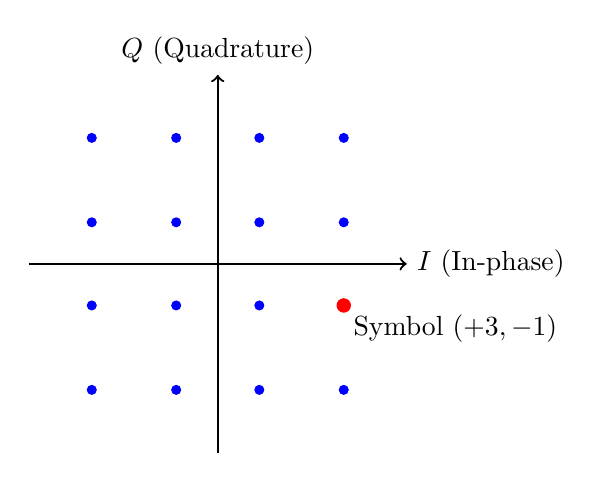
\begin{tikzpicture}[scale=0.8]
    % Draw axes
    \draw[->, thick] (-3,0) -- (3,0) node[right] {$I$ (In-phase)};
    \draw[->, thick] (0,-3) -- (0,3) node[above] {$Q$ (Quadrature)};
    
    % Draw 16-QAM points as a simplified visualization
    \foreach \x in {-2, -0.66, 0.66, 2}
        \foreach \y in {-2, -0.66, 0.66, 2}
            \filldraw[blue] (\x,\y) circle (2pt);
            
    % Highlight one point
    \filldraw[red] (2,-0.66) circle (3pt) node[anchor=north west, black] {Symbol $(+3, -1)$};
\end{tikzpicture}
\caption{Visualization of a QAM Constellation Grid mapping $I$ and $Q$ values.}
\label{fig:qam_constellation}
\end{figure}

\subsection{\textbf{Transmission and Symbol Mapping}}
In an operational QAM transmitter, an incoming bitstream (e.g., \texttt{110101 001011 111000}) is segmented into groups. Each group maps to a single constellation point defined by a predetermined mapping table. 

Assuming a specific data segment \texttt{101011} maps to the coordinates $I = +3$ and $Q = -1$, the transmitted signal $s(t)$ is formulated as:
\begin{equation}
    s(t) = I \cos(2\pi f_c t) + Q \sin(2\pi f_c t)
\end{equation}
Different bit combinations produce distinct waveforms, ensuring unique symbols are transmitted across the channel.


\subsection{\textbf{Signal Extraction at the Receiver}}
At the receiver, the goal is to map the incoming waveform back to a constellation point by extracting the $I$ and $Q$ values.

\begin{enumerate}
    \item \textbf{I-Extraction:} The received signal is multiplied by $\cos(2\pi f_c t)$ and passed through an integrator (averaging filter). Because sine and cosine are orthogonal over a full period, this process nullifies the $Q$ component and isolates the $I$ magnitude.
    \item \textbf{Q-Extraction:} The signal is multiplied by $\sin(2\pi f_c t)$ and averaged, which eliminates the $I$ component and isolates $Q$.
\end{enumerate}

Due to channel noise, the extracted values will rarely be perfect integers. Suppose the processing yields $I \approx 3.1$ and $Q \approx -0.8$. A decision boundary algorithm maps this back to the nearest valid constellation point $(3, -1)$, which is then demodulated back into the bit sequence \texttt{101011}.

\subsection{\textbf{Adaptive Modulation and Noise Trade-offs}}
Higher-order modulations exponentially increase the data rate, but suffer from increased susceptibility to noise.

\begin{table}[h]
\centering
\caption{Modulation Schemes and Data Rates}
\begin{tabular}{lcc}
\toprule
\textbf{Modulation} & \textbf{Symbols} & \textbf{Bits / Symbol} \\
\midrule
BPSK  & 2   & 1 \\
QPSK  & 4   & 2 \\
16-QAM & 16  & 4 \\
64-QAM & 64  & 6 \\
256-QAM & 256 & 8 \\
\bottomrule
\end{tabular}
\end{table}

In robust schemes like QPSK, the constellation points are physically separated by larger Euclidean distances, meaning the channel noise must be exceptionally high to force a symbol into an adjacent decision region. Conversely, in dense constellations like 64-QAM or 256-QAM, the points are packed closely together, making them highly sensitive to interference.

To optimize throughput while maintaining acceptable Bit Error Rates (BER), modern transceivers employ \textbf{Adaptive Modulation}. If the Signal-to-Noise Ratio (SNR) drops, the system dynamically downshifts the modulation order (e.g., $64\text{-QAM} \to 16\text{-QAM} \to \text{QPSK}$) to prioritize connection stability over peak data rate.


\section{\large \textbf{The Bandwidth Crunch and the Paradigm Shift}}
As modern wireless networks transition toward 6G, data demands are scaling exponentially. Emergent technologies such as autonomous vehicles, Augmented Reality/Virtual Reality (AR/VR), and digital twins require an unprecedented volume of data transmission. However, physical bandwidth remains strictly limited, and transmitting every individual bit across the network has become unsustainably expensive.

Conventional systems are fundamentally bound by the necessity to transmit raw data streams, attempting to reconstruct the exact binary sequence at the receiver side. Yet, modern network data contains immense structural redundancy. While traditional communication insists on sending every single bit with absolute numerical accuracy, the actual semantic meaning or core intent of the message is often orders of magnitude smaller than the raw bitstream representation. 

To demonstrate the boundaries of classical physical layer scaling, Table~\ref{tab:network_specs} outlines the performance metrics across frequency ranges (FR1 and FR2) alongside historical baselines. Despite massive expansions in bandwidth and the deployment of higher subcarrier spacing (SCS), the spectral efficiency ($bit/s/Hz$) fundamentally saturates. This bottleneck underscores the necessity of a architectural shift from bit-level replication to semantic preservation.

% FIX: Changed from table to table* so it spans across both columns neatly without overlapping text
\begin{table*}[t]
\centering
\caption{Physical Layer Throughput and Efficiency Performance Metrics}
\label{tab:network_specs}
\begin{tabular}{lcccccc}
\toprule
\textbf{Frequency Range} & \textbf{SCS} & \textbf{Bandwidth} & \textbf{DL Throughput} & \textbf{UL Throughput} & \textbf{Efficiency DL} & \textbf{Efficiency UL} \\
\midrule
FR1 & 15 kHz & 50 MHz & 288.9 Mbit/s & 309.1 Mbit/s & 5.78 bit/s/Hz & 6.18 bit/s/Hz \\
FR1 & 30 kHz & 100 MHz & 584.3 Mbit/s & 625.0 Mbit/s & 5.84 bit/s/Hz & 6.25 bit/s/Hz \\
FR1 & 60 kHz & 100 MHz & 577.8 Mbit/s & 618.1 Mbit/s & 5.78 bit/s/Hz & 6.18 bit/s/Hz \\
FR2 & 60 kHz & 200 MHz & 1.08 Gbit/s & 1.18 Gbit/s & 5.40 bit/s/Hz & 5.90 bit/s/Hz \\
FR2 & 120 kHz & 400 MHz & 2.15 Gbit/s & 2.37 Gbit/s & 5.38 bit/s/Hz & 5.93 bit/s/Hz \\
\midrule
\textbf{Comparison with LTE} & & & & & & \\
All bands & 15 kHz & 20 MHz & 100 Mbit/s & 100 Mbit/s & 5.00 bit/s/Hz & 5.00 bit/s/Hz \\
\midrule
\textbf{Comparison with 3G} & & & & & & \\
All bands & - & 5 MHz & 21.1 Mbit/s & 17.2 Mbit/s & 4.22 bit/s/Hz & 3.44 bit/s/Hz \\
\bottomrule
\end{tabular}
\end{table*}

\section{\large \textbf{Architecture of a Semantic Communication System}}
To bypass the limitations of Shannon’s traditional framework, a semantic layer is integrated directly into the transceiving pipeline. Instead of translating raw sequences to bits, the system extracts the vital objects, actions, deep intent, meaning, and contextual background of the data, transmitting exclusively this compressed semantic essence.

\subsection{\textbf{End-to-End System Block Diagram}}
The operational framework replaces standard source components with intelligent deep learning blocks that interface directly with localized and global knowledge bases. 

% FIX: Changed from figure to figure* to span both columns and redesigned the TikZ layout to be perfectly neat
\begin{figure*}[t]
\centering
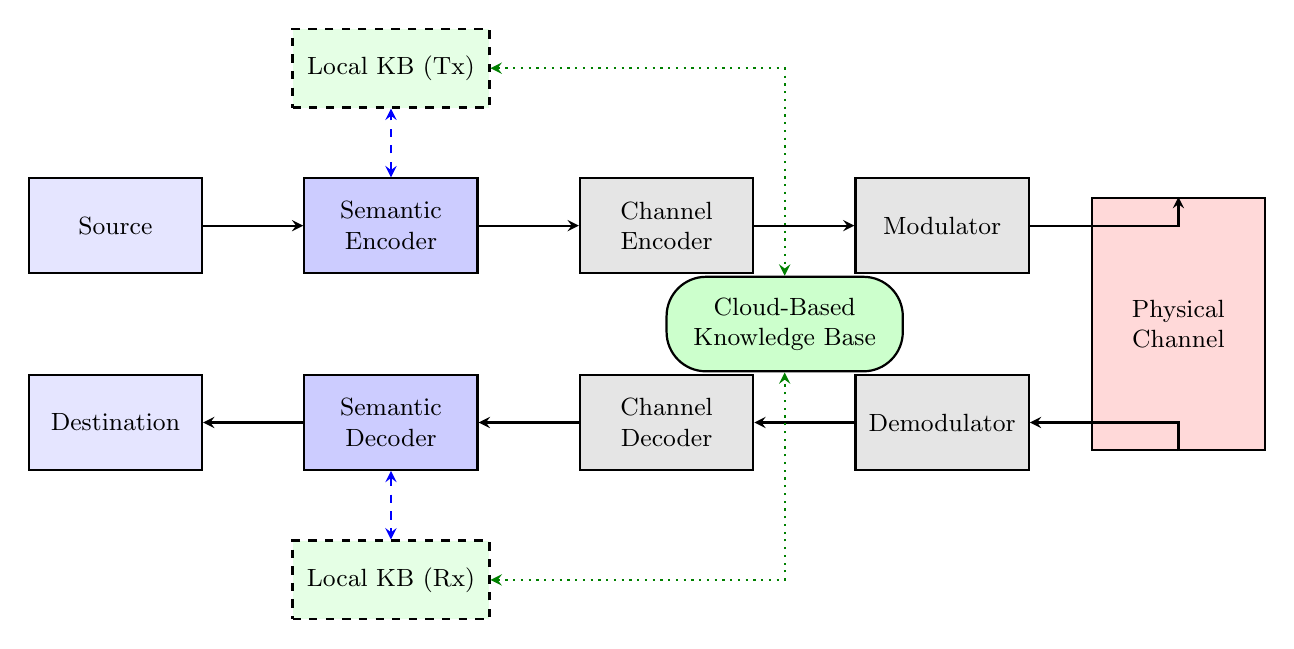
\begin{tikzpicture}[
    >=stealth,
    block/.style={draw, rectangle, fill=blue!10, minimum height=1.2cm, minimum width=2.2cm, align=center, font=\small, thick},
    kb/.style={draw, dashed, rectangle, fill=green!10, minimum height=1cm, minimum width=2.5cm, align=center, font=\small, thick},
    cloud/.style={draw, rectangle, fill=green!20, rounded corners=0.5cm, minimum height=1.2cm, minimum width=3cm, align=center, font=\small, thick}
]

    % Tx nodes
    \node[block] (src) at (0,0) {Source};
    \node[block, fill=blue!20] (se) at (3.5,0) {Semantic\\Encoder};
    \node[block, fill=gray!20] (ce) at (7,0) {Channel\\Encoder};
    \node[block, fill=gray!20] (mod) at (10.5,0) {Modulator};

    % Channel node
    \node[block, fill=red!15, minimum height=3.2cm] (ch) at (13.5,-1.25) {Physical\\Channel};

    % Rx nodes
    \node[block] (dest) at (0,-2.5) {Destination};
    \node[block, fill=blue!20] (sd) at (3.5,-2.5) {Semantic\\Decoder};
    \node[block, fill=gray!20] (cd) at (7,-2.5) {Channel\\Decoder};
    \node[block, fill=gray!20] (demod) at (10.5,-2.5) {Demodulator};

    % Knowledge Bases
    \node[kb] (lkb1) at (3.5, 2) {Local KB (Tx)};
    \node[kb] (lkb2) at (3.5, -4.5) {Local KB (Rx)};
    \node[cloud] (ckb) at (8.5, -1.25) {Cloud-Based\\Knowledge Base};

    % Connections Top
    \draw[->, thick] (src) -- (se);
    \draw[->, thick] (se) -- (ce);
    \draw[->, thick] (ce) -- (mod);
    \draw[->, thick] (mod.east) -| (ch.north);
    
    % Connections Bottom
    \draw[->, thick] (ch.south) |- (demod.east);
    \draw[->, thick] (demod) -- (cd);
    \draw[->, thick] (cd) -- (sd);
    \draw[->, thick] (sd) -- (dest);

    % KB links
    \draw[<->, thick, blue, dashed] (se) -- (lkb1);
    \draw[<->, thick, blue, dashed] (sd) -- (lkb2);
    
    % Cloud links
    \draw[<->, thick, green!50!black, dotted] (lkb1.east) -| (ckb.north);
    \draw[<->, thick, green!50!black, dotted] (lkb2.east) -| (ckb.south);

\end{tikzpicture}
\caption{System architecture of an intelligent semantic communication framework utilizing synchronized shared knowledge bases.}
\label{fig:semantic_architecture}
\end{figure*}

Modern implementations of these semantic components utilize advanced artificial intelligence architectures, such as Transformers, BERT, and deep Autoencoders. These models are uniquely capable of learning highly dense, low-dimensional mathematical representations of human language and environment states.

\subsection{\textbf{Paradigm Comparison Matrix}}
The shift from classical communication to semantic architecture changes the fundamental metrics used to evaluate system performance, as contrasted in Table~\ref{tab:paradigm_comparison}.

\begin{table}[h]
\centering
\caption{System Metrics and Paradigms Comparison}
\label{tab:paradigm_comparison}
\begin{tabular}{lll}
\toprule
\textbf{Parameter} & \textbf{Traditional Communication} & \textbf{Semantic Communication} \\
\midrule
\textbf{Transmission Core} & Raw binary bits & Underlying data meaning \\
\textbf{System Focus} & Structural accuracy of sequence & Realized intent of message \\
\textbf{Primary Metric} & Bit Error Rate (BER) & Semantic similarity index \\
\textbf{Theoretical Basis} & Shannon Information Theory & AI-driven Semantic Theory \\
\textbf{Context Treatment} & Meaning + Context + Redundancy & Meaning alone \\
\bottomrule
\end{tabular}
\end{table}

\section{\large \textbf{Shared Knowledge Bases and Graph Representations}}

\subsection{\textbf{Knowledge Base Synchronization}}
A foundational requirement for semantic communication is the synchronization of knowledge. The transmitting agent ($Tx$) and receiving agent ($Rx$) must share a structurally consistent understanding of the application domain prior to transmission. This relationship is governed by the shared knowledge base constraint:
\begin{equation}
    \text{SKB}_{Tx} \approx \text{SKB}_{Rx}
\end{equation}
The Shared Knowledge Base (SKB) acts as a comprehensive common repository, encapsulating domain-specific ontologies, structured knowledge graphs, explicit localized facts, semantic text embeddings, contextual relationship maps between diverse entities, and pre-trained language model parameters.

\subsection{\textbf{Knowledge Graph-Based Representations}}
Semantic communication frameworks rely heavily on highly structured semantic representations. A knowledge graph organizes real-world entities and maps the explicit relationships connecting them, translating disjoint data points into a cohesive relational network that provides deep situational context. Information within a knowledge graph is formally structured into discrete relational triplets:
\begin{equation}
    \text{Triplet} = \big(\text{Entity}_1, \, \text{Relation}, \, \text{Entity}_2\big)
\end{equation}

\begin{figure}[h]
\centering
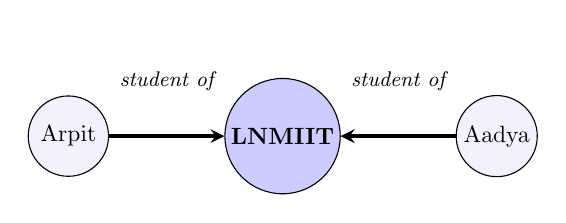
\begin{tikzpicture}[node distance=2.5cm, auto, >=stealth, every node/.style={circle, draw, fill=blue!5, minimum size=1.2cm, inner sep=2pt}, scale=0.85, transform shape]
    \node (lnmiit) [fill=blue!20, font=\bfseries] {LNMIIT};
    \node (arpit) [left of=lnmiit, node distance=3.2cm] {Arpit};
    \node (aadya) [right of=lnmiit, node distance=3.2cm] {Aadya};

    \draw [->, thick, line width=1.2pt] (arpit) -- node[above, draw=none, fill=none, font=\small\itshape] {student of} (lnmiit);
    \draw [->, thick, line width=1.2pt] (aadya) -- node[above, draw=none, fill=none, font=\small\itshape] {student of} (lnmiit);
\end{tikzpicture}
\caption{A sample structural knowledge graph demonstrating entity-relation mapping.}
\label{fig:knowledge_graph}
\end{figure}

\section{\large \textbf{Semantic Encoding and Decoding Mechanics}}

\subsection{\textbf{Semantic Encoding}}
Instead of treating text as a stream of characters to be processed by standard source encoders, an NLP module parses raw text sequences into distinct entities, relations, and attributes. These relational triplets are then mapped directly into dense vector spaces via deep learning models. 

The resulting high-dimensional semantic vector captures the contextual intent using significantly fewer total bits than would be required if the original sentence were translated into text characters and expanded using traditional error-correcting block codes.

\subsection{\textbf{Semantic Decoding}}
Upon receiving the channel-degraded vector embedding, the receiver does not execute bit-by-bit error correction. Instead, the decoding block combines the incoming semantic vector with its localized Shared Knowledge Base ($SKB_{Rx}$) to feed an intelligent language generation model. 

While the syntactical structure of the newly generated sentence may visually differ from the original input text, the semantic content, core message, and human intent are preserved perfectly.

\section{\large \textbf{Channel Noise Resilience and Probabilistic Inference}}

\subsection{\textbf{Traditional Error Overhead}}
In a traditional physical layer setup, when a channel disturbance corrupts transmitted bits, the data packets fail their respective integrity checks (e.g., CRC). Consequently, a retransmission request is generated across the link via Automatic Repeat Request (ARQ) protocols. This introduces significant system vulnerabilities:
\begin{itemize}
    \item Substantial increases in overall processing latency.
    \item Higher instantaneous channel bandwidth consumption.
    \item Pronounced degradation in end-to-end network efficiency.
\end{itemize}

\subsection{\textbf{Semantic Error Mitigation via Inference}}
Conversely, semantic communication frameworks demonstrate innate resilience against channel noise. If the received vector representation of a knowledge graph triplet suffers corruption during transmission, the receiver can leverage the strong structural priors embedded within its localized knowledge base ($SKB_{Rx}$).

Consider an illustrative scenario where an edge agent transmits engineering context, and a key node in the semantic graph sequence is corrupted:
\begin{equation}
    \big(\text{VLSI}, \, \text{subject of}, \, \underline{\text{? [Corrupted]}}\big)
\end{equation}
Because the synchronized knowledge base contains deep contextual domain mapping, the receiver does not request a retransmission. Instead, it applies probabilistic reasoning across its existing network paths to evaluate the missing structural component, immediately inferring that the corrupted term refers to \textit{Signals/Systems}. 

Errors are resolved through native receiver-side \textbf{Inference} rather than channel-dependent \textbf{Retransmission}, estimating the lost information accurately without requiring additional channel resources. This framework provides a viable pathway for ultra-reliable, low-latency execution across 6G networks, Edge AI systems, and autonomous vehicle arrays.

\section{\large \textbf{Machine Learning and Deep Learning Integration in Semantic Communication}}

\subsection{\textbf{Transmitting Meaning Rather Than Bits}}
In traditional communication, information is represented as symbols and bits, and performance is analyzed using metrics such as Bit Error Rate (BER) and Signal-to-Noise Ratio (SNR). The shift towards semantic communication introduces a new paradigm: transmitting meaning rather than bits.

However, this introduces a significant challenge: semantic meaning is highly complex, context-dependent, and subjective. There is no standard mathematical expression for ``meaning.'' Designing an algorithm to extract semantic components—such as object, action, intent, and relation—is extremely difficult. For unstructured data like images, videos, and audio, this complexity further increases. Determining which component is semantically important for transmission is not straightforward. Hardcoded, rule-based mathematical models are impractical. This limitation strongly motivates the integration of Machine Learning (ML) and Deep Learning (DL) techniques.

\subsection{\textbf{Deep Learning as a Semantic Encoder}}
Neural networks trained on large datasets replace manually designed feature extraction. The objective is to learn a compressed representation. The semantic encoder receives raw data (such as text, speech, image, and video) and transforms it:

\begin{equation}
    Z = f_\theta(X)
\end{equation}

Where:
\begin{itemize}
    \item $X$ is the raw input data.
    \item $f_\theta$ is a neural network parameterized by weights $\theta$.
    \item $Z$ is a semantic embedding containing the most relevant information.
\end{itemize}

The transmitter sends this learned semantic representation $Z$, ensuring that the core meaning is preserved across the transmission.

\begin{figure}[h]
\centering
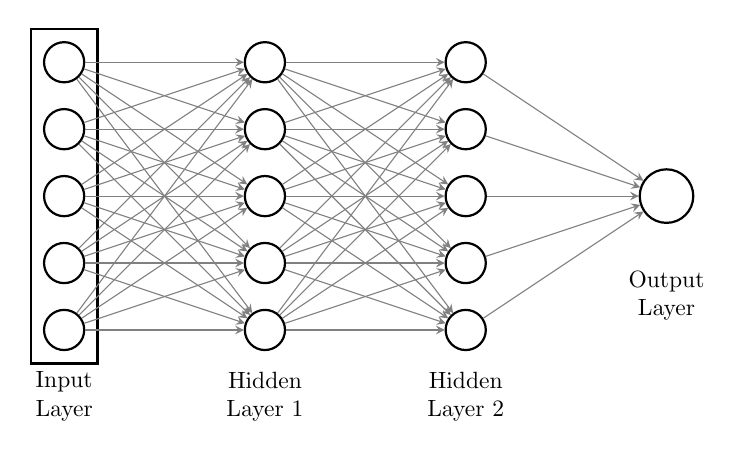
\begin{tikzpicture}[>=stealth, scale=0.85, every node/.style={transform shape}]
    % Input Layer
    \foreach \i in {1,...,5}
        \node[circle, draw, thick, minimum size=0.6cm] (I\i) at (0, 3-\i) {};
    \node[align=center, below] at (0, -2.5) {Input\\Layer};
    \draw[thick] (-0.5, 2.5) rectangle (0.5, -2.5);

    % Hidden Layer 1
    \foreach \i in {1,...,5}
        \node[circle, draw, thick, minimum size=0.6cm] (H1\i) at (3, 3-\i) {};
    \node[align=center, below] at (3, -2.5) {Hidden\\Layer 1};

    % Hidden Layer 2
    \foreach \i in {1,...,5}
        \node[circle, draw, thick, minimum size=0.6cm] (H2\i) at (6, 3-\i) {};
    \node[align=center, below] at (6, -2.5) {Hidden\\Layer 2};

    % Output Layer
    \node[circle, draw, thick, minimum size=0.8cm] (O) at (9, 0) {};
    \node[align=center, below] at (9, -1) {Output\\Layer};

    % Connections
    \foreach \i in {1,...,5}
        \foreach \j in {1,...,5}
            \draw[->, gray] (I\i) -- (H1\j);

    \foreach \i in {1,...,5}
        \foreach \j in {1,...,5}
            \draw[->, gray] (H1\i) -- (H2\j);

    \foreach \i in {1,...,5}
        \draw[->, gray] (H2\i) -- (O);
\end{tikzpicture}
\caption{Neural network acting as a semantic encoder transforming input data into an output embedding.}
\label{fig:nn_encoder}
\end{figure}

\subsection{\textbf{Neural Networks in Semantic Communication}}
A neural network is a computational model that learns a mapping between inputs and outputs by adjusting internal parameters through training. The learned transformation can be expressed as:
\begin{equation}
    y = f(x)
\end{equation}

\subsubsection{\textbf{Mathematical Model of a Neuron}}
Consider an artificial neuron receiving multiple inputs: $x_1, x_2, x_3, \dots, x_n$. Each input has an associated weight: $w_1, w_2, w_3, \dots, w_n$.
The neuron computes the weighted sum:
\begin{equation}
    z = x_1w_1 + x_2w_2 + \dots + x_nw_n + b
\end{equation}
Expressed in vector notation:
\begin{equation}
    z = w^T x + b
\end{equation}
The result is then passed to an activation function to produce the output $a$:
\begin{equation}
    a = \phi(z) = \phi(w^T x + b)
\end{equation}

\textbf{Example Calculation:}\\
Given inputs $x = [2, 3]$, weights $w = [0.5, 0.8]$, and bias $b = 1$:
\begin{equation}
    z = (2)(0.5) + (3)(0.8) + 1 = 1 + 2.4 + 1 = 4.4
\end{equation}
Applying the ReLU activation function $\phi(z) = \max(0, z)$:
\begin{equation}
    a = \max(0, 4.4) = 4.4
\end{equation}
This final value $a$ represents the neuron output.

\subsection{\textbf{Role of Activation Function}}
Without an activation function, a neural network is just a large linear equation. Real-world semantic relationships are non-linear. The activation function introduces this vital non-linearity into the system. Common activation functions include:
\begin{itemize}
    \item \textbf{Sigmoid:} $\sigma(x) = \frac{1}{1 + e^{-x}}$, where $0 < \sigma(x) < 1$
    \item \textbf{Tanh:} $\tanh(x)$, where $-1 < \tanh(x) < 1$
    \item \textbf{ReLU:} $\text{ReLU}(x) = \max(0, x)$
\end{itemize}

\subsection{\textbf{Layer Organization and Feature Abstraction}}
Neurons are organized into distinct layers to process information hierarchically:
\begin{itemize}
    \item \textbf{Input Layer:} Receives raw information.
    \item \textbf{Hidden Layers:} Perform feature extraction and abstraction. Lower layers learn simple patterns, while higher layers learn complex concepts.
    \item \textbf{Output Layer:} Produces semantic embeddings, classifications, or predictions.
\end{itemize}

For example, in text processing:
\begin{figure}[h]
\centering
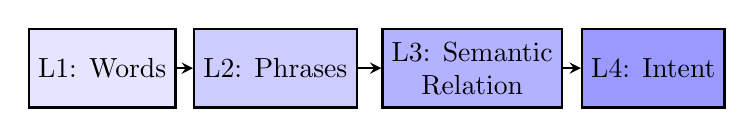
\begin{tikzpicture}[>=stealth, auto, node distance=2cm, thick]
    \node[draw, rectangle, minimum height=1cm, minimum width=1.5cm, fill=blue!10] (L1) {L1: Words};
    \node[draw, rectangle, minimum height=1cm, minimum width=1.5cm, fill=blue!20, right of=L1, node distance=2.2cm] (L2) {L2: Phrases};
    \node[draw, rectangle, minimum height=1cm, minimum width=1.8cm, fill=blue!30, right of=L2, node distance=2.5cm, align=center] (L3) {L3: Semantic\\Relation};
    \node[draw, rectangle, minimum height=1cm, minimum width=1.5cm, fill=blue!40, right of=L3, node distance=2.3cm] (L4) {L4: Intent};

    \draw[->] (L1) -- (L2);
    \draw[->] (L2) -- (L3);
    \draw[->] (L3) -- (L4);
\end{tikzpicture}
\caption{Hierarchical abstraction of text across neural network layers.}
\label{fig:layer_abstraction}
\end{figure}

\subsection{\textbf{Training and Gradient Descent}}
Initially, the network's weights are random. The network gradually improves by comparing its predictions against correct answers. The objective is to minimize the Loss Function $L(y, \hat{y})$.

Through Gradient Descent, the network adjusts weights to reduce this loss:
\begin{equation}
    w_{new} = w_{old} - \eta \frac{\partial L}{\partial w}
\end{equation}
Where $\eta$ represents the learning rate. This process is repeated millions of times during training. Eventually, the network discovers useful semantic patterns hidden within the data. After passing through multiple layers, the network transforms raw data into a compact numerical representation known as an embedding:
\begin{equation}
    Z = [z_1, z_2, \dots, z_n]
\end{equation}

\subsection{\textbf{The Semantic Communication Pipeline}}
In this ML-integrated architecture, the standard transmitter and receiver modules are replaced by semantic counterparts.

\begin{itemize}
    \item \textbf{Semantic Encoder:} Maps the message to an embedding ($\text{Message} \rightarrow \text{Embedding}$).
    \item \textbf{Semantic Decoder:} Maps the embedding back to meaning ($\text{Embedding} \rightarrow \text{Meaning}$).
\end{itemize}

\begin{figure}[h]
\centering
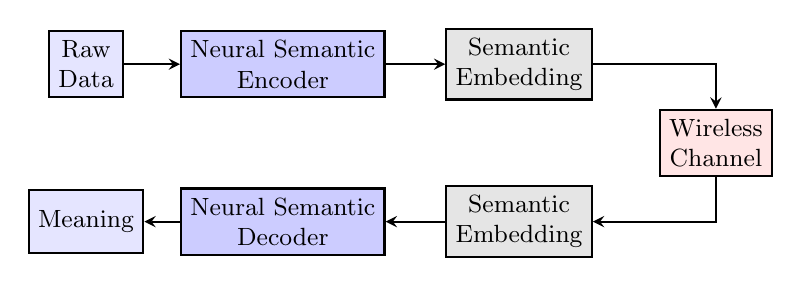
\begin{tikzpicture}[>=stealth, thick,
    block/.style={draw, rectangle, fill=blue!10, minimum height=0.8cm, align=center, font=\small},
    channel/.style={draw, rectangle, fill=red!10, minimum height=0.8cm, align=center, font=\small}]

    \node[block] (raw) at (0,0) {Raw\\Data};
    \node[block, fill=blue!20] (enc) at (2.5,0) {Neural Semantic\\Encoder};
    \node[block, fill=gray!20] (emb1) at (5.5,0) {Semantic\\Embedding};
    \node[channel] (ch) at (8, -1) {Wireless\\Channel};
    \node[block, fill=gray!20] (emb2) at (5.5,-2) {Semantic\\Embedding};
    \node[block, fill=blue!20] (dec) at (2.5,-2) {Neural Semantic\\Decoder};
    \node[block] (mean) at (0,-2) {Meaning};

    \draw[->] (raw) -- (enc);
    \draw[->] (enc) -- (emb1);
    \draw[->] (emb1.east) -| (ch.north);
    \draw[->] (ch.south) |- (emb2.east);
    \draw[->] (emb2) -- (dec);
    \draw[->] (dec) -- (mean);
\end{tikzpicture}
\caption{End-to-End Semantic Communication Pipeline using Neural Networks.}
\label{fig:semantic_pipeline}
\end{figure}

\section{\large \textbf{Numerical Analysis of Deep Learning Models}}

\subsection{\textbf{Forward Propagation with a Single Hidden Neuron}}
To understand how semantic representations are learned, it is essential to trace the mathematical operations during a forward pass. Consider a simple neural network with an input layer of 2 neurons and an output layer of 1 neuron, utilizing a single hidden neuron with a Rectified Linear Unit (ReLU) activation function.

Let the inputs be $x_1 = 2$ and $x_2 = 3$, with a true target value of $y = 10$. The network initializes with the following random weights and biases:
\begin{itemize}
    \item Hidden layer weights: $w_1 = 0.5$, $w_2 = 0.8$
    \item Hidden layer bias: $b_h = 1$
    \item Output layer weight: $v = 1.2$
    \item Output layer bias: $b_o = 0$
\end{itemize}

The pre-activation value at the hidden neuron, $z_h$, is computed as:
\begin{align}
    z_h &= w_1x_1 + w_2x_2 + b_h \\
    z_h &= (0.5)(2) + (0.8)(3) + 1 \\
    z_h &= 1 + 2.4 + 1 = 4.4
\end{align}

Applying the ReLU activation function, $a_h = \max(0, z_h)$:
\begin{equation}
    a_h = \max(0, 4.4) = 4.4
\end{equation}

Moving to the output neuron, the predicted value $\hat{y}$ is computed:
\begin{align}
    \hat{y} &= v a_h + b_o \\
    \hat{y} &= (1.2)(4.4) + 0 = 5.28
\end{align}

The error in this prediction is measured using the Mean Squared Error (MSE) loss function:
\begin{align}
    L &= \frac{1}{2}(y - \hat{y})^2 \\
    L &= \frac{1}{2}(10 - 5.28)^2 = 11.1392
\end{align}

\subsection{\textbf{Backpropagation and Weight Optimization}}
To improve the network's prediction, the weights must be updated using gradient descent. The first step is to calculate the gradient of the loss with respect to the output prediction:
\begin{equation}
    \frac{\partial L}{\partial \hat{y}} = (\hat{y} - y) = (5.28 - 10) = -4.72
\end{equation}
The negative sign indicates that the current prediction is too low compared to the true value.

Next, we update the output weight $v$. The gradient is computed via the chain rule:
\begin{equation}
    \frac{\partial L}{\partial v} = (\hat{y} - y) a_h = (-4.72)(4.4) = -20.768
\end{equation}

Given a learning rate $\eta = 0.01$, the new output weight is:
\begin{align}
    v_{new} &= v - \eta \frac{\partial L}{\partial v} \\
    v_{new} &= 1.2 - 0.01(-20.768) = 1.40768
\end{align}

Similarly, we update the hidden weights $w_1$ and $w_2$. The gradient for $w_1$ requires passing the error through the ReLU derivative:
\begin{equation}
    \frac{\partial L}{\partial w_1} = (\hat{y} - y) \times v \times \text{ReLU}'(z_h) \times x_1
\end{equation}
Since $z_h = 4.4 > 0$, the derivative $\text{ReLU}'(4.4) = 1$.
\begin{equation}
    \frac{\partial L}{\partial w_1} = (-4.72)(1.2)(1)(2) = -11.328
\end{equation}
The updated weight $w_1$ becomes:
\begin{equation}
    w_1 = 0.5 - 0.01(-11.328) = 0.61328
\end{equation}

Following the same process for $w_2$:
\begin{align}
    \frac{\partial L}{\partial w_2} &= (-4.72)(1.2)(1)(3) = -16.992 \\
    w_2 &= 0.8 - 0.01(-16.992) = 0.96992
\end{align}

\subsection{\textbf{Iterative Semantic Learning}}
After a single forward and backward pass, the network parameters have shifted, resulting in a prediction much closer to the target value.

\begin{table}[h]
\centering
\begin{tabular}{|c|c|}
\hline
\textbf{Before Training} & \textbf{After 1 Iteration} \\ \hline
$w_1 = 0.5$ & $w_1 \approx 0.61$ \\
$w_2 = 0.8$ & $w_2 \approx 0.96$ \\
$v = 1.2$ & $v \approx 1.4$ \\
$a_h = 4.4$ & $a_h = 5.13$ \\
$\hat{y} = 5.28$ & $\hat{y} = 7.23 \rightarrow \text{Closer to 10}$ \\ \hline
\end{tabular}
\caption{Parameter adjustments after one cycle of gradient descent.}
\label{tab:weight_update}
\end{table}

After millions of training examples consisting of forward passes, loss computations, backpropagation, and weight updates, the network eventually learns abstract semantic relationships, such as recognizing that "car" $\approx$ "vehicle" and "fast" $\approx$ "speed".

\section{\large \textbf{Transformer Architectures in Semantic Communication}}

\subsection{\textbf{The Self-Attention Mechanism}}
While traditional recurrent neural networks process data sequentially, Transformer architectures introduce the concept of self-attention. This allows neural networks to capture long-range semantic relationships within data. Unlike recurrent networks, a transformer can simultaneously analyze all components of an input sequence and determine their relative importance.

For an input sequence $X = \{x_1, x_2, \dots, x_n\}$, the model computes the mathematical relationship between every possible pair of elements. The resulting attention weights dictate which parts of the input contribute most significantly to the overall semantic meaning of the message. For example, in the sentence "neural networks is a great concept of machine learning," the attention mechanism strongly connects "neural networks" to "machine learning."

\begin{figure}[h]
\centering
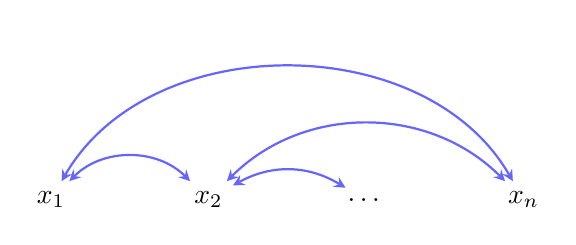
\begin{tikzpicture}[>=stealth, auto, node distance=1.5cm, thick]
    \node (x1) at (0,0) {$x_1$};
    \node (x2) at (2,0) {$x_2$};
    \node (dots) at (4,0) {$\dots$};
    \node (xn) at (6,0) {$x_n$};

    \draw[<->, bend left=45, blue!60] (x1) to (x2);
    \draw[<->, bend left=60, blue!60] (x1) to (xn);
    \draw[<->, bend left=45, blue!60] (x2) to (xn);
    \draw[<->, bend left=30, blue!60] (x2) to (dots);
\end{tikzpicture}
\caption{Self-attention mechanism computing pairwise semantic relationships simultaneously across the entire input sequence.}
\label{fig:self_attention}
\end{figure}

\subsection{\textbf{Generative AI for Semantic Reconstruction}}
In modern semantic frameworks, Generative AI plays a critical role at the receiver end. The receiver utilizes a semantic decoder $g_\phi$ to reconstruct the original intent of the message from the transmitted semantic embedding $Z$. The reconstructed message $\hat{X}$ is formulated as:
\begin{equation}
    \hat{X} = g_\phi(Z)
\end{equation}
In this generative process, the exact wordings may differ from the original input, but the core context and meaning remain identical.

\begin{figure}[h]
\centering

\resizebox{\columnwidth}{!}{
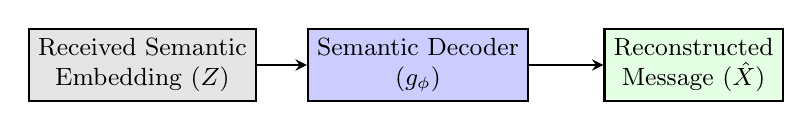
\begin{tikzpicture}[
    >=stealth,
    thick,
    block/.style={
        draw,
        rectangle,
        fill=blue!10,
        minimum height=0.8cm,
        minimum width=2.2cm,
        align=center,
        font=\small
    }
]

    % Nodes
    \node[block, fill=gray!20] (z) at (0,0)
    {Received Semantic\\Embedding ($Z$)};

    \node[block, fill=blue!20] (decoder) at (3.5,0)
    {Semantic Decoder\\($g_\phi$)};

    \node[block, fill=green!10] (xhat) at (7,0)
    {Reconstructed\\Message ($\hat{X}$)};

    % Arrows
    \draw[->] (z) -- (decoder);
    \draw[->] (decoder) -- (xhat);

\end{tikzpicture}
}

\caption{Semantic reconstruction utilizing Generative AI at the receiver.}
\label{fig:gen_ai_reconstruction}

\end{figure}

\section{\large \textbf{Performance Metrics in Semantic Systems}}

\subsection{\textbf{Inadequacy of Traditional Metrics}}
In standard communication frameworks, performance is heavily evaluated based on exact signal reconstruction metrics. These include:
\begin{itemize}
    \item \textbf{Bit Error Rate (BER):} $\frac{\text{Number of incorrect bits}}{\text{Total number of bits}}$
    \item \textbf{Symbol Error Rate (SER):} $\frac{\text{Incorrect symbols}}{\text{Total symbols}}$
    \item \textbf{Packet Error Rate (PER):} $\frac{\text{Corrupted packets}}{\text{Total packets}}$
\end{itemize}

These metrics fundamentally assume that absolute exactness in signal reconstruction is required. However, semantic communication allows for syntactic modification. As a result, metrics like BER may indicate a significant error or failure even when the fundamental meaning of the transmitted message remains completely unchanged. 

\subsection{\textbf{Semantic Evaluation: The BLEU Score}}
To effectively measure semantic preservation, metrics from natural language processing are adapted. One prominent metric is the BLEU (Bilingual Evaluation Understudy) score. 

The BLEU score measures the overlap between the generated reconstructed text and the original reference text using $n$-gram matching techniques. A higher score indicates a stronger similarity between the strings. 
\begin{equation}
    \text{BLEU} \in [0, 1]
\end{equation}

While BLEU is a step forward, it primarily evaluates literal word similarity and $n$-gram overlaps. Consequently, it may still fail to capture deeper semantic equivalence where entirely different vocabulary is used to perfectly convey the same meaning, highlighting the ongoing need for advanced semantic evaluation metrics.

\section{\large \textbf{Semantic Evaluation Metrics in NLP}}

As semantic communication shifts the focus from bit-level accuracy to intent preservation, evaluating the performance of these systems requires specialized metrics derived from Natural Language Processing (NLP). This chapter outlines the foundational methodologies for quantifying semantic similarity and translation quality.

\subsection{\textbf{N-gram Matching}}
An $n$-gram is defined as a contiguous sequence of $n$ items (typically words) extracted from a given text sequence. They are fundamental in analyzing the structural composition of sentences.

\begin{itemize}
    \item \textbf{Unigrams ($n=1$):} Capture the raw vocabulary of the text.
    \item \textbf{Higher-order N-grams ($n>1$):} Capture sentence structure and localized context. The higher the order of the $n$-gram, the better it captures semantic relations.
\end{itemize}

Given a sample sentence: \textit{"I lost my mind, no one noticed"}, the extraction yields:
\begin{itemize}
    \item \textbf{Unigram ($n=1$):} \{I, lost, my, mind, no, one\}
    \item \textbf{Bigram ($n=2$):} \{I lost, lost my, my mind, mind no\}
    \item \textbf{Trigram ($n=3$):} \{I lost my, lost my mind, \dots\}
\end{itemize}

\begin{figure}[h]
\centering
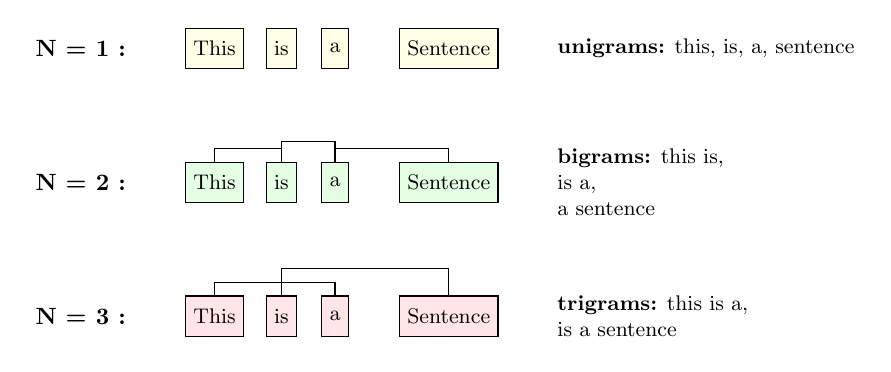
\begin{tikzpicture}[
    box/.style={draw, rectangle, minimum height=0.6cm, font=\small, align=center},
    scale=0.85, transform shape
]
    % Unigrams
    \node[font=\bfseries] at (-2, 2) {N = 1 :};
    \node[box, fill=yellow!10] (u1) at (0,2) {This};
    \node[box, fill=yellow!10] (u2) at (1,2) {is};
    \node[box, fill=yellow!10] (u3) at (1.8,2) {a};
    \node[box, fill=yellow!10] (u4) at (3.5,2) {Sentence};
    \node[right, font=\small] at (5, 2) {\textbf{unigrams:} this, is, a, sentence};

    % Bigrams
    \node[font=\bfseries] at (-2, 0) {N = 2 :};
    \node[box, fill=green!10] (b1) at (0,0) {This};
    \node[box, fill=green!10] (b2) at (1,0) {is};
    \node[box, fill=green!10] (b3) at (1.8,0) {a};
    \node[box, fill=green!10] (b4) at (3.5,0) {Sentence};
    \draw (b1.north) -- ++(0,0.2) -| (b2.north);
    \draw (b2.north) -- ++(0,0.3) -| (b3.north);
    \draw (b3.north) -- ++(0,0.2) -| (b4.north);
    \node[right, font=\small, align=left] at (5, 0) {\textbf{bigrams:} this is,\\ is a,\\ a sentence};

    % Trigrams
    \node[font=\bfseries] at (-2, -2) {N = 3 :};
    \node[box, fill=red!10] (t1) at (0,-2) {This};
    \node[box, fill=red!10] (t2) at (1,-2) {is};
    \node[box, fill=red!10] (t3) at (1.8,-2) {a};
    \node[box, fill=red!10] (t4) at (3.5,-2) {Sentence};
    \draw (t1.north) -- ++(0,0.2) -| (t3.north);
    \draw (t2.north) -- ++(0,0.4) -| (t4.north);
    \node[right, font=\small, align=left] at (5, -2) {\textbf{trigrams:} this is a,\\ is a sentence};
\end{tikzpicture}
\caption{Visualization of continuous N-gram sequencing applied to a sample sentence.}
\label{fig:ngrams}
\end{figure}

\subsection{\textbf{BLEU Score Evaluation}}
The Bilingual Evaluation Understudy (BLEU) score primarily measures \textit{precision} by calculating how many generated phrases appear sequentially in the reference text.

The BLEU metric is formulated as:
\begin{equation}
    \text{BLEU} = \text{BP} \cdot \exp\left( \sum_{n=1}^{N} w_n \log p_n \right)
\end{equation}
Where:
\begin{itemize}
    \item $N = 4$ (Standard maximum $n$-gram limit)
    \item $w_n = \text{Weighting factor}$
    \item $p_n = n\text{-gram precision}$
\end{itemize}

\subsubsection{\textbf{Brevity Penalty (BP)}}
A critical component of BLEU is the Brevity Penalty, which prevents the system from unfairly rewarding extremely short, high-precision generations that miss broader semantic context. Consider the following:
\begin{itemize}
    \item \textbf{Reference:} \textit{the college is good}
    \item \textbf{Generated:} \textit{the college}
\end{itemize}
Although the precision is exceptionally high, vital information is omitted. To combat this, the penalty is calculated as:
\begin{equation}
    \text{BP} = e^{\left(1 - \frac{r}{c}\right)}
\end{equation}
where $c$ is the candidate length and $r$ is the reference length.

\subsubsection{\textbf{Advantages and Limitations}}
\begin{table}[h]
\centering
\caption{BLEU Score Characteristics}
\begin{tabular}{p{4cm}p{4cm}}
\toprule
\textbf{Advantages} & \textbf{Limitations} \\
\midrule
Easy and efficient to compute & Primarily measures word overlap \\
Highly effective for machine translation & Fails to capture deeper semantic meaning \\
\bottomrule
\end{tabular}
\end{table}

\begin{figure}[h]
\centering
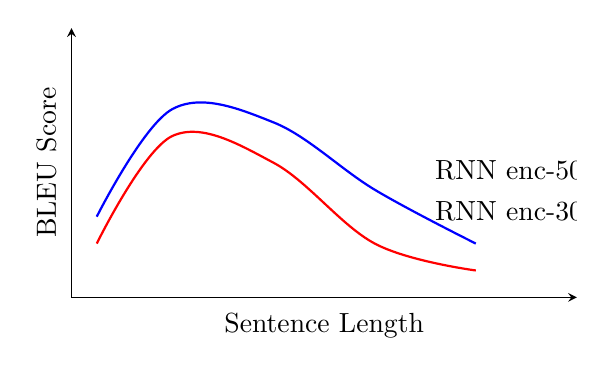
\begin{tikzpicture}
\begin{axis}[
    width=8cm, height=5cm,
    xlabel={Sentence Length},
    ylabel={BLEU Score},
    xmin=0, xmax=100,
    ymin=0, ymax=100,
    xtick=\empty, ytick=\empty,
    axis lines=left,
    every axis plot/.append style={thick}
]
% Simulating the handwritten graph trajectories
\addplot[smooth, tension=0.6, blue] coordinates {(5,30) (20,70) (40,65) (60,40) (80,20)};
\node[anchor=south west] at (axis cs:70,40) {RNN enc-50};

\addplot[smooth, tension=0.6, red] coordinates {(5,20) (20,60) (40,50) (60,20) (80,10)};
\node[anchor=south west] at (axis cs:70,25) {RNN enc-30};
\end{axis}
\end{tikzpicture}
\caption{Effect of sequence length on BLEU performance across varying encoder parameters.}
\label{fig:bleu_graph}
\end{figure}

\subsection{\textbf{ROUGE Score}}
In contrast to BLEU's precision focus, ROUGE (Recall-Oriented Understudy for Gisting Evaluation) is fundamentally recall-oriented. It evaluates how much of the original reference information successfully appears within the generated text.

\subsubsection{\textbf{ROUGE-N}}
This metric measures the raw matching of $n$-grams between the candidate and the reference:
\begin{equation}
    \text{ROUGE}_N = \frac{\text{matching } n\text{-grams}}{\text{reference } n\text{-grams}}
\end{equation}

\subsubsection{\textbf{ROUGE-L}}
ROUGE-L leverages the Longest Common Subsequence (LCS) to score the text. Instead of relying on consecutive matches, it identifies the longest co-occurring sequence of words. This approach natively rewards the structural maintenance of the sequence without requiring strict, contiguous $n$-gram overlap.

\section{\large \textbf{Transformers Foundation in Semantic Communication}}

\subsection{\textbf{Evaluation Metrics: BLEU vs ROGUE}}
In evaluating generated textual representations within semantic structures, it is essential to distinguish between the primary metrics utilized for scoring.

\begin{table}[h]
\centering
\caption{Comparison of BLEU and ROGUE Metrics}
\label{tab:bleu_vs_rogue}
\begin{tabular}{lcc}
\toprule
\textbf{Attribute} & \textbf{BLEU} & \textbf{ROGUE} \\
\midrule
\textbf{Focus} & Precision & Recall \\
\textbf{Popular in} & Translation & Summarization \\
\textbf{Denominator} & Generated text words & Reference text words \\
\textbf{Penalizes extra words} & $\checkmark$ & $\times$ \\
\textbf{Penalizes missing words} & $\times$ & $\checkmark$ \\
\bottomrule
\end{tabular}
\end{table}

\subsection{\textbf{Limitations of Previous Architectures}}
Before the advent of transformers, classical architectures faced significant limitations in handling sequence data and semantic continuity:
\begin{itemize}
    \item \textbf{Feedforward Neural Networks (FFN):} An FFN treats every input independently. Given an input vector $x = [x_1, x_2, x_3, x_4]$, there is no mechanism to understand word order, context, or long-range dependency.
    \item \textbf{Recurrent Neural Networks (RNN):} RNNs introduced memory into the architecture:
    \begin{equation}
        h_t = f(x_t, h_{t-1})
    \end{equation}
    where $x_t$ is the current word and $h_t$ is the hidden state. While the hidden state successfully carried information forward, long sentences ultimately lost information due to the vanishing gradient problem.
\end{itemize}

Transformers eliminate recurrence entirely. In a transformer framework, every word directly examines every other word—a mechanism fundamentally known as \textit{Self-Attention}.

\subsection{\textbf{Input Processing and Positional Encoding}}
In a transformer, each word is converted into a vector. Because transformers process all words simultaneously, they inherently lack sequential awareness and require explicit position information. 

Positional Encoding (PE) is injected using sine and cosine functions:
\begin{equation}
    PE(pos, 2i) = \sin\left(\frac{pos}{10000^{2i/d}}\right)
\end{equation}
\begin{equation}
    PE(pos, 2i+1) = \cos\left(\frac{pos}{10000^{2i/d}}\right)
\end{equation}
where $d$ represents the embedding dimension. The final embedding fed into the network is the combination of these factors:
\begin{equation}
    \text{Embedding} = \text{word vector} + \text{position}
\end{equation}

\subsection{\textbf{The Self-Attention Mechanism}}
Every embedded word generates three distinct vectors via learnable weight matrices ($W_Q, W_K, W_V$):
\begin{align}
    \text{Query (Q)} &= X W_Q \\
    \text{Key (K)} &= X W_K \\
    \text{Value (V)} &= X W_V
\end{align}

To understand this conceptually through an analogy:
\begin{itemize}
    \item \textbf{Query:} The text you type in a search bar.
    \item \textbf{Key:} Titles, tags, and metadata of all candidate videos.
    \item \textbf{Value:} The actual video you watch, once a match is found.
\end{itemize}

The core interaction is determined by the \textbf{Attention Score}, calculated as $Q K^T$. For example, given $Q = [2, 1]$ and $K = [3, 2]$, the score is $Q K^T = (2)(3) + (1)(2)$.

\subsubsection{\textbf{Scaling and Softmaxing}}
Calculating the raw attention score alone can result in a large vector with unstable values. To mitigate this, the score undergoes \textbf{Scaling}:
\begin{equation}
    \text{Scaled Score} = \frac{Q K^T}{\sqrt{d_k}}
\end{equation}
where $d_k$ is the key dimension.

Following scaling, \textbf{Softmaxing} is applied to convert the scores into normalized probabilities:
\begin{equation}
    \text{Softmax}(x_i) = \frac{e^{x_i}}{\sum e^{x_j}}
\end{equation}
This ensures that $\sum_i \text{attention} = 1$. For example, an unnormalized score array of $[8, 2, 1]$ becomes $[0.995, 0.004, 0.001]$, clearly indicating that the first word holds the vast majority of the importance.

The final output is the attention map multiplied by the Value ($V$):
\begin{equation}
    Z = \sum \alpha_i V_i
\end{equation}
The complete, unified attention equation is formalized as:
\begin{equation}
    \text{Attention}(Q, K, V) = \text{softmax}\left(\frac{Q K^T}{\sqrt{d_k}}\right) V
\end{equation}

\subsection{\textbf{Multi-Head Attention}}
A single attention mechanism focuses on only one relationship. Transformers, therefore, use multiple attention heads. Different heads learn different semantic relations across the text sequence.

\begin{equation}
    \text{Head}_i = \text{Attention}(Q_i, K_i, V_i)
\end{equation}
\begin{equation}
    \text{MultiHead} = \text{Concat}(\text{Head}_1, \dots, \text{Head}_n)
\end{equation}

\begin{figure}[h]
\centering
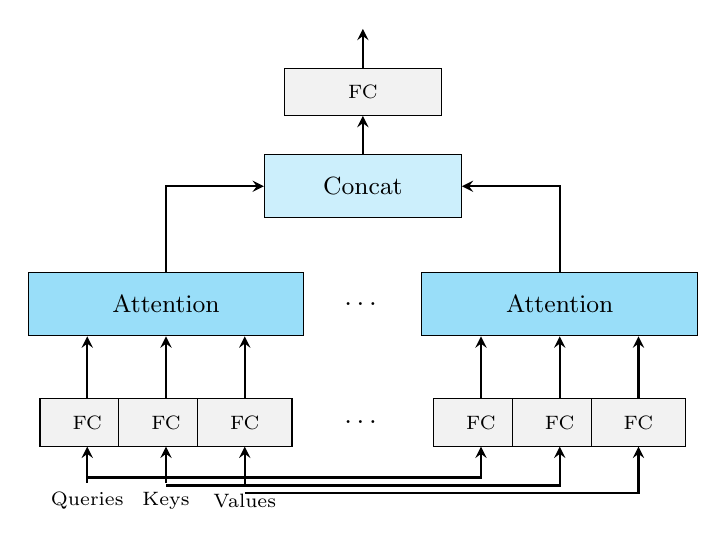
\begin{tikzpicture}[
    >=stealth,
    box/.style={draw, rectangle, minimum height=0.6cm, minimum width=1.2cm, align=center, fill=gray!10, font=\scriptsize},
    attn/.style={draw, rectangle, minimum height=0.8cm, minimum width=3.5cm, align=center, fill=cyan!40, font=\small},
    concat/.style={draw, rectangle, minimum height=0.8cm, minimum width=2.5cm, align=center, fill=cyan!20, font=\small}
]

% Inputs
\node (q) at (-2.5, 0) {\scriptsize Queries};
\node (k) at (-1.5, 0) {\scriptsize Keys};
\node (v) at (-0.5, 0) {\scriptsize Values};

\node (q2) at (2.5, 0) {}; 
\node (k2) at (3.5, 0) {}; 
\node (v2) at (4.5, 0) {};

% Linear Layers (FC)
\node[box] (fc1) at (-2.5, 1) {FC};
\node[box] (fc2) at (-1.5, 1) {FC};
\node[box] (fc3) at (-0.5, 1) {FC};

\node[box] (fc4) at (2.5, 1) {FC};
\node[box] (fc5) at (3.5, 1) {FC};
\node[box] (fc6) at (4.5, 1) {FC};

% Attention Blocks
\node[attn] (attn1) at (-1.5, 2.5) {Attention};
\node[attn] (attn2) at (3.5, 2.5) {Attention};

% Dots
\node at (1, 1) {\dots};
\node at (1, 2.5) {\dots};

% Concat and Final FC
\node[concat] (concat) at (1, 4) {Concat};
\node[box, minimum width=2cm] (fcout) at (1, 5.2) {FC};

% Connections Layer 1
\draw[->, thick] (q) -- (fc1);
\draw[->, thick] (k) -- (fc2);
\draw[->, thick] (v) -- (fc3);

% Connections branching to second set
\draw[->, thick] (-2.5,0.3) -| (fc4);
\draw[->, thick] (-1.5,0.2) -| (fc5);
\draw[->, thick] (-0.5,0.1) -| (fc6);

% Connections to Attention
\draw[->, thick] (fc1) -- (attn1.south -| fc1);
\draw[->, thick] (fc2) -- (attn1.south -| fc2);
\draw[->, thick] (fc3) -- (attn1.south -| fc3);

\draw[->, thick] (fc4) -- (attn2.south -| fc4);
\draw[->, thick] (fc5) -- (attn2.south -| fc5);
\draw[->, thick] (fc6) -- (attn2.south -| fc6);

% Connections to Concat
\draw[->, thick] (attn1) |- (concat);
\draw[->, thick] (attn2) |- (concat);

% Final Output
\draw[->, thick] (concat) -- (fcout);
\draw[->, thick] (fcout) -- +(0,0.8);

\end{tikzpicture}
\caption{Structural workflow of Multi-Head Attention, utilizing multiple linear projections (FC) and parallel Attention computation blocks.}
\label{fig:multihead}
\end{figure}

\subsection{\textbf{Feed-Forward Networks and Layer Normalization}}
After processing through the attention mechanism, each token passes through a Feed-Forward Network (FFN) to allow non-linear semantic transformation:
\begin{equation}
    FFN(x) = W_2(\text{ReLU}(W_1 x + b_1)) + b_2
\end{equation}

To ensure training stability and to prevent exploding activations within the deep network, Layer Normalization ($x$) is applied:
\begin{equation}
    \text{LayerNorm} = \frac{(x - \mu)}{\sqrt{\sigma^2 + \epsilon}}
\end{equation}

\subsection{\textbf{Cosine Similarity}}
In semantic vector spaces, similarity is calculated using Cosine Similarity, computing the normalized dot product of two vectors, $A = [a_1, a_2, \dots, a_n]$ and $B = [b_1, b_2, \dots, b_n]$:
\begin{equation}
    \text{CosSim} = \frac{A \cdot B}{|A||B|}
\end{equation}
where the dot product and magnitude are derived as:
\begin{align}
    A \cdot B &= \sum a_i b_i \\
    |A| &= \sqrt{\sum a_i^2}
\end{align}

\section{\large \textbf{Transformer Architecture and Deep Learning Integration}}

This chapter details the fundamental deep learning structures utilized in the semantic processing of information, specifically focusing on the Transformer architecture and its core component, the Multi-Head Attention mechanism.

\subsection{\textbf{The Transformer Architecture}}
The Transformer framework relies heavily on self-attention mechanisms to process sequential data, discarding the need for recurrent structures. It consists of an encoder block that processes the input sequence and a decoder block that generates the output sequence.

\begin{figure}[htbp]
\centering
\resizebox{\columnwidth}{!}{%
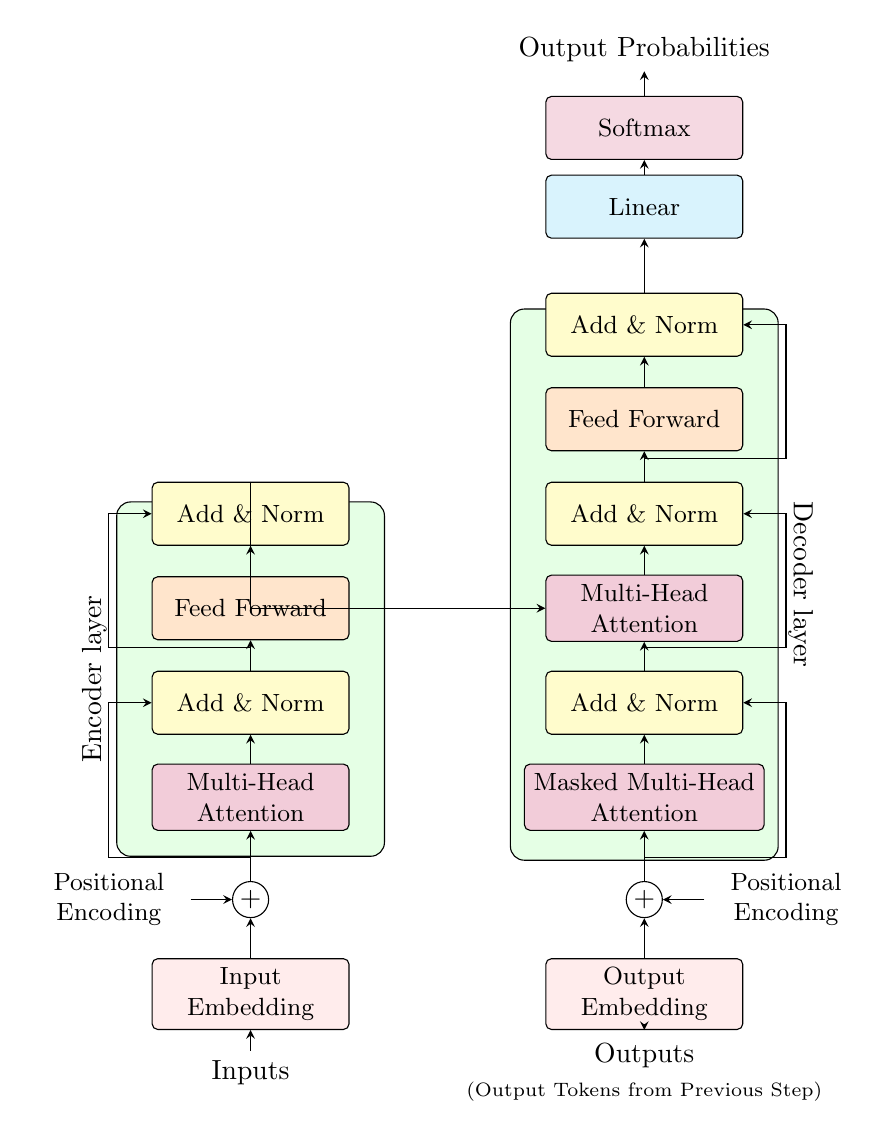
\begin{tikzpicture}[
    >=stealth,
    box/.style={draw, rectangle, rounded corners=2pt, minimum width=2.5cm, minimum height=0.8cm, align=center, font=\small},
    pinkbox/.style={box, fill=pink!30},
    yellowbox/.style={box, fill=yellow!20},
    orangebox/.style={box, fill=orange!20},
    bluebox/.style={box, fill=cyan!20},
    purplebox/.style={box, fill=purple!20},
    encdec/.style={draw, rectangle, rounded corners=5pt, fill=green!10, minimum width=3.4cm, inner sep=10pt}
]

    % Encoder Side
    \node (input) at (0,0) {Inputs};
    \node[pinkbox] (in_emb) at (0,1) {Input\\Embedding};
    \node[circle, draw, inner sep=1pt] (add1) at (0,2.2) {$+$};
    \node (pos_enc1) at (-1.8,2.2) {\small \begin{tabular}{c} Positional \\ Encoding \end{tabular}};
    \draw[->] (pos_enc1) -- (add1);

    % Encoder Block
    \node[encdec, minimum height=4.5cm] (encoder) at (0, 5) {};
    \node[left] at (encoder.west) {\rotatebox{90}{Encoder layer}};

    \node[purplebox] (mha1) at (0, 3.5) {Multi-Head\\Attention};
    \node[yellowbox] (an1) at (0, 4.7) {Add \& Norm};
    \node[orangebox] (ff1) at (0, 5.9) {Feed Forward};
    \node[yellowbox] (an2) at (0, 7.1) {Add \& Norm};

    \draw[->] (input) -- (in_emb);
    \draw[->] (in_emb) -- (add1);
    \draw[->] (add1) -- (mha1);
    \draw[->] (mha1) -- (an1);
    \draw[->] (an1) -- (ff1);
    \draw[->] (ff1) -- (an2);

    % Residuals Encoder
    \draw[->] (add1.north) -- ++(0,0.3) -| ++(-1.8,0) |- (an1.west);
    \draw[->] (an1.north) -- ++(0,0.3) -| ++(-1.8,0) |- (an2.west);

    % Decoder Side
    \node (output) at (5,0) {\begin{tabular}{c} Outputs \\ \scriptsize (Output Tokens from Previous Step) \end{tabular}};
    \node[pinkbox] (out_emb) at (5,1) {Output\\Embedding};
    \node[circle, draw, inner sep=1pt] (add2) at (5,2.2) {$+$};
    \node (pos_enc2) at (6.8,2.2) {\small \begin{tabular}{c} Positional \\ Encoding \end{tabular}};
    \draw[->] (pos_enc2) -- (add2);

    % Decoder Block
    \node[encdec, minimum height=7cm] (decoder) at (5, 6.2) {};
    \node[right] at (decoder.east) {\rotatebox{-90}{Decoder layer}};

    \node[purplebox] (mmha) at (5, 3.5) {Masked Multi-Head\\Attention};
    \node[yellowbox] (an3) at (5, 4.7) {Add \& Norm};
    \node[purplebox] (mha2) at (5, 5.9) {Multi-Head\\Attention};
    \node[yellowbox] (an4) at (5, 7.1) {Add \& Norm};
    \node[orangebox] (ff2) at (5, 8.3) {Feed Forward};
    \node[yellowbox] (an5) at (5, 9.5) {Add \& Norm};

    \draw[->] (output) -- (out_emb);
    \draw[->] (out_emb) -- (add2);
    \draw[->] (add2) -- (mmha);
    \draw[->] (mmha) -- (an3);
    \draw[->] (an3) -- (mha2);
    \draw[->] (mha2) -- (an4);
    \draw[->] (an4) -- (ff2);
    \draw[->] (ff2) -- (an5);

    % Cross Attention Link
    \draw[->] (an2.north) |- (mha2.west);

    % Residuals Decoder
    \draw[->] (add2.north) -- ++(0,0.3) -| ++(1.8,0) |- (an3.east);
    \draw[->] (an3.north) -- ++(0,0.3) -| ++(1.8,0) |- (an4.east);
    \draw[->] (an4.north) -- ++(0,0.3) -| ++(1.8,0) |- (an5.east);

    % Output Layers
    \node[bluebox, fill=cyan!15] (linear) at (5, 11) {Linear};
    \node[purplebox, fill=purple!15] (softmax) at (5, 12) {Softmax};
    \node (out_prob) at (5, 13) {Output Probabilities};

    \draw[->] (an5) -- (linear);
    \draw[->] (linear) -- (softmax);
    \draw[->] (softmax) -- (out_prob);

\end{tikzpicture}
}
\caption{Systematic representation of the Transformer Architecture, illustrating the interconnected Encoder and Decoder pipelines.}
\label{fig:transformer_structure}
\end{figure}

\subsection{\textbf{Multi-Head Attention Mechanism}}
The Multi-Head Attention component resolves long-range dependencies by allowing the model to jointly attend to information from disparate representation subspaces across different sequential positions. The process formally segments the input Queries (Q), Keys (K), and Values (V) into multiple parallel computation heads before evaluating the attention weights and systematically recombining the output.

\begin{figure}[htbp]
\centering
\resizebox{\columnwidth}{!}{%
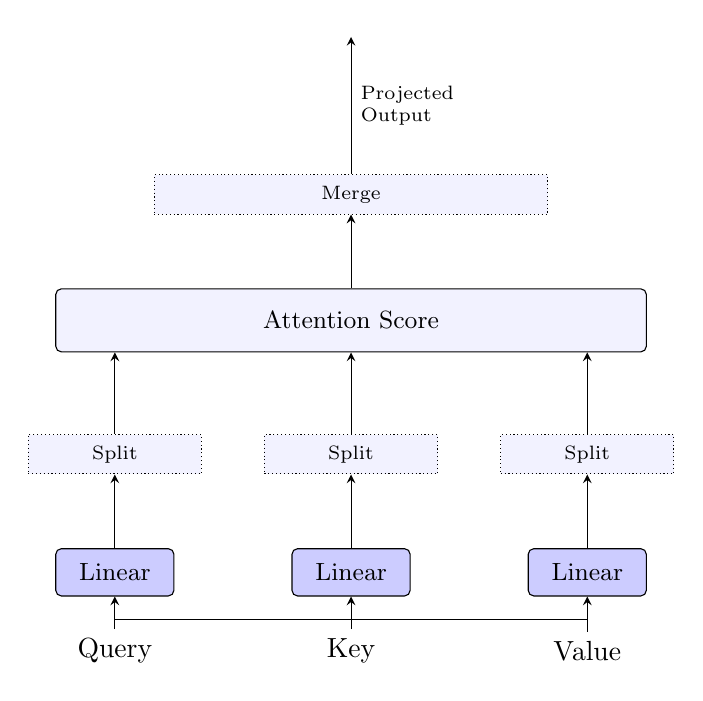
\begin{tikzpicture}[
    >=stealth,
    box/.style={draw, rectangle, rounded corners=2pt, minimum width=1.5cm, minimum height=0.6cm, align=center, font=\small},
    bluebox/.style={box, fill=blue!20},
    graybox/.style={box, fill=blue!5, minimum width=7.5cm, minimum height=0.8cm},
    splitbox/.style={draw, densely dotted, rectangle, fill=blue!5, minimum width=2.2cm, minimum height=0.5cm, align=center, font=\scriptsize}
]

    % Inputs
    \node (q_in) at (-3,0) {Query};
    \node (k_in) at (0,0) {Key};
    \node (v_in) at (3,0) {Value};

    % Linear Projections
    \node[bluebox] (lin_q) at (-3,1) {Linear};
    \node[bluebox] (lin_k) at (0,1) {Linear};
    \node[bluebox] (lin_v) at (3,1) {Linear};

    \draw[->] (q_in) -- (lin_q);
    \draw[->] (k_in) -- (lin_k);
    \draw[->] (v_in) -- (lin_v);
    \draw[-] (-3, 0.4) -- (0, 0.4);
    \draw[-] (0, 0.4) -- (3, 0.4);

    % Split Representations
    \node[splitbox] (split_q) at (-3,2.5) {Split};
    \node[splitbox] (split_k) at (0,2.5) {Split};
    \node[splitbox] (split_v) at (3,2.5) {Split};

    \draw[->] (lin_q) -- (split_q);
    \draw[->] (lin_k) -- (split_k);
    \draw[->] (lin_v) -- (split_v);

    % Attention Score Integration
    \node[graybox] (attn) at (0,4.2) {Attention Score};

    \draw[->] (split_q) -- (attn.south -| split_q);
    \draw[->] (split_k) -- (attn.south -| split_k);
    \draw[->] (split_v) -- (attn.south -| split_v);

    % Merge Box
    \node[splitbox, minimum width=5cm] (merge) at (0,5.8) {Merge};
    \draw[->] (attn) -- (merge);

    % Final Linear Output
    \node (output_lbl) at (0, 7.8) {}; 
    \draw[->] (merge) -- (output_lbl.center) node[midway, right, align=left, font=\scriptsize] {Projected\\Output};

\end{tikzpicture}
}
\caption{Detailed schematic of the Multi-Head Attention Mechanism, illustrating the segmentation and subsequent merging of the Q, K, and V tensors.}
\label{fig:multi_head_attention}
\end{figure}

\section{\large \textbf{Transformer Architecture for Semantic Communication}}

\subsection{\textbf{Step 1: Input Embedding}}
The first step maps discrete input tokens into continuous dense vectors.
\begin{equation}
    x_i \in \mathbb{R}^{d_{model}}
\end{equation}
For example, an input representation could be: $x = [0.7, 0.2, -0.3, 0.9]$.

\subsection{\textbf{Step 2: Positional Encoding}}
To inject sequence order information into the model, positional encodings are added to the input embeddings.
\begin{equation}
    E_i = x_i + PE_i
\end{equation}
Where the positional encoding (PE) is defined using sine and cosine functions of different frequencies:
\begin{align}
    PE(pos, 2i) &= \sin\left(\frac{pos}{10000^{2i/d}}\right) \\
    PE(pos, 2i+1) &= \cos\left(\frac{pos}{10000^{2i/d}}\right)
\end{align}

\subsection{\textbf{Step 3: Encoder Layer}}
The encoder runs $N$ times. Each encoder layer has a fundamental repeating structure: 
\textit{Multi-Head Attention} $\rightarrow$ \textit{Add \& Normalize} $\rightarrow$ \textit{Feed Forward} $\rightarrow$ \textit{Add \& Normalize}.

\subsection{\textbf{Step 4: Self Multi-Head Attention}}
The self-attention mechanism derives the Query ($Q$), Key ($K$), and Value ($V$) matrices from the embedded input $X$.
\begin{equation}
    X = [E_1, E_2, \dots, E_n]
\end{equation}
\begin{align}
    Q &= XW_Q \\
    K &= XW_K \\
    V &= XW_V
\end{align}

Suppose $X = \begin{bmatrix} 1 & 2 \\ 3 & 4 \end{bmatrix}$. This makes $Q, K, V$ vectors by the formulas. The attention score between token $i$ and token $j$ is:
\begin{equation}
    \text{score}_{ij} = Q_i K_j^T
\end{equation}
This measures relevance using the concept of multi-head attention. Let $i = 2$ and $Q_2$, then compare with every key vector $K$ ($K_1, K_2, K_3, K_4, K_5, K_6$). Compute all scores:
\begin{equation}
    Q_2K_1^T, Q_2K_2^T, Q_2K_3^T, Q_2K_4^T, \dots, Q_2K_6^T
\end{equation}
Find all the scores over attention after softmaxing you'll get top related words. Now vary $i$ and $j$ for all $e \in X, Q, K$.

\subsection{\textbf{Step 5 \& 6: Scaling and Softmax}}
\textbf{Step 5 (Scaling):} The dot product is scaled to prevent vanishing gradients:
\begin{equation}
    \frac{Q_i K_j^T}{\sqrt{d_k}}
\end{equation}
\textbf{Step 6 (Softmax):} Convert scores to probabilities:
\begin{equation}
    \alpha_{ij} = \frac{e^{\text{score}_{ij}}}{\sum_j e^{\text{score}_{ij}}}
\end{equation}
Where $0 \leq \alpha_{ij} \leq 1$ and $\sum_j \alpha_{ij} = 1$. The final output $Z_i$ is computed as:
\begin{equation}
    Z_i = \sum_j \alpha_{ij} V_j
\end{equation}
Every token contains info from all other tokens.

\subsection{\textbf{Step 7: Multi-Head Attention}}
Instead of one attention mechanism, $h_1, h_2, \dots, h_m$ multiple attention heads with separate $W_Q, W_K, W_V$ matrices are used.
\begin{equation}
    \text{Multihead} = \text{Concat}(\text{head}_1, \dots, \text{head}_m) W_O
\end{equation}

\subsection{\textbf{Step 8: Add and Norm \& Feed Forward Network}}
\textbf{Add and Norm:} 
Let $Y = \text{Attention}(X)$. The residual connection and normalization is applied as:
\begin{equation}
    Y_1 = \text{LayerNorm}(X + Y)
\end{equation}
Here, $X$ is the input and $Y$ is the learned transformation. This enables deeper networks by preventing vanishing gradients.
\begin{equation}
    \text{LayerNorm}(x) = \frac{x - \mu}{\sqrt{\sigma^2 + \epsilon}}
\end{equation}
This ensures activation stays stable.

\textbf{Feed Forward Network:} A small neural network applied to every token:
\begin{equation}
    FFN(x) = W_2(\text{ReLU}(W_1x + b_1)) + b_2
\end{equation}
Suppose $W_1 = \begin{bmatrix} 1 & 0 \\ 0 & 1 \end{bmatrix}$ and $x = [2, 3]$, with $W_2 = \begin{bmatrix} 2 & 0 \\ 0 & 2 \end{bmatrix}$. 
Then $W_1x = [2, 3]$ and $W_2x = [4, 6]$. This allows non-linear feature extraction.

\subsection{\textbf{Step 9 \& 10: Encoder Output}}
\textbf{Step 9 (Add and normalize again):}
\begin{equation}
    Y_2 = \text{LayerNorm}(Y_1 + FFN(Y_1))
\end{equation}
This completes one encoder layer. The output is passed into the next encoder layer. After many layers, the sequence transforms from word embedding $\rightarrow$ attention layers $\rightarrow$ contextual embeddings.

\textbf{Step 10 (Encoder output):}
Eventually, $H = [h_1, h_2, \dots, h_n]$. These vectors contain contextual information.

\begin{figure}[h]
\centering
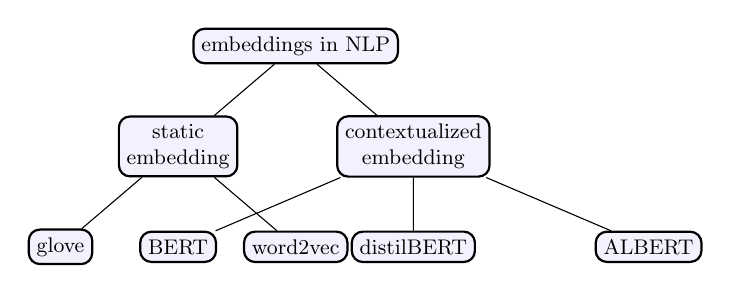
\begin{tikzpicture}[sibling distance=10em,
  every node/.style = {shape=rectangle, rounded corners, draw, align=center, fill=blue!5, thick, font=\small}, scale=0.85, transform shape]
  \node {embeddings in NLP}
    child { node {static\\embedding}
      child { node {glove} }
      child { node {word2vec} } }
    child { node {contextualized\\embedding}
      child { node {BERT} }
      child { node {distilBERT} }
      child { node {ALBERT} } };
\end{tikzpicture}
\caption{Classification of static and contextualized NLP embeddings.}
\label{fig:embeddings_nlp}
\end{figure}

\subsection{\textbf{Step 11: Decoder Input}}
The decoder receives:
\begin{itemize}
    \item Encoder output $H$
    \item Previously generated tokens
\end{itemize}

\subsection{\textbf{Step 12: Masked Multi-Head Attention}}
This is the same as self-attention except future tokens are hidden. A mask matrix $M$ is added, so that future words can't be seen from encoder output.
\begin{equation}
    \text{attention} = \text{SoftMax}\left( \frac{QK^T}{\sqrt{d_k}} + M \right)
\end{equation}

\subsection{\textbf{Step 13: Encoder - Decoder Attention}}
In this layer:
\begin{align*}
    Q &= \text{Decoder} \\
    K, V &= \text{Encoder}
\end{align*}
This allows the decoder to focus on relevant encoder information.

\subsection{\textbf{Step 14: Feed Forward + Add \& Normalize + Linear Layer}}
The output is passed through a feed-forward layer:
\begin{equation}
    FFN(x) = W_2(\text{RELU}(W_1x + b_1))
\end{equation}
For the linear layer, the decoder output $\rightarrow h$.
Then $z = Wh + b$. The output dimension is $|vocab|$. 
If there are 50000 words, then $z \in \mathbb{R}^{50000}$. Each element is a score for one possible word.

\subsection{\textbf{Step 15: Softmax}}
Convert score to probabilities. The highest probability is choosen.
\begin{equation}
    P(\text{word}_i) = \frac{e^{z_i}}{\sum_j e^{z_j}}
\end{equation}

\section{\large \textbf{Semantic Communication Architecture}}
The Transformer encoder-decoder architecture seamlessly maps sequence intent. Input tokens $\rightarrow$ encoder $\rightarrow$ contextual semantic representation $\rightarrow$ decoder $\rightarrow$ output tokens.

\begin{figure}[h]
\centering
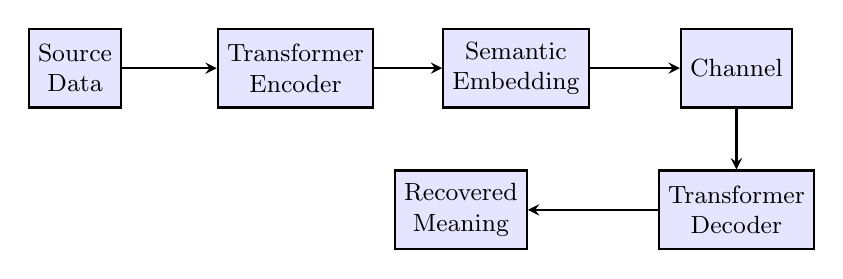
\begin{tikzpicture}[>=stealth, auto, node distance=2.2cm,
    block/.style={draw, rectangle, fill=blue!10, minimum height=1cm, text centered, font=\small, thick, align=center}]
    \node[block] (src) {Source\\Data};
    \node[block, right of=src, node distance=2.8cm] (enc) {Transformer\\Encoder};
    \node[block, right of=enc, node distance=2.8cm] (emb) {Semantic\\Embedding};
    \node[block, right of=emb, node distance=2.8cm] (chan) {Channel};
    \node[block, below of=chan, node distance=1.8cm] (dec) {Transformer\\Decoder};
    \node[block, left of=dec, node distance=3.5cm] (rec) {Recovered\\Meaning};

    \draw[->, thick] (src) -- (enc);
    \draw[->, thick] (enc) -- (emb);
    \draw[->, thick] (emb) -- (chan);
    \draw[->, thick] (chan) -- (dec);
    \draw[->, thick] (dec) -- (rec);
\end{tikzpicture}
\caption{Semantic communication data flow mapping meaning directly over a channel.}
\label{fig:semantic_comm_flow}
\end{figure}
\section{\large \textbf{Joint Source Channel Coding (JSCC)}}

\subsection{\textbf{Limitations of Traditional Systems}}
In traditional communication systems, source coding and channel coding are designed independently based on the separation principle, provided that the source coding rate is less than the channel capacity ($R_s < C$). However, Shannon's theorem fundamentally assumes infinite block lengths, unlimited computational resources, and perfect encoding. 

Modern applications such as autonomous vehicles, Internet of Things (IoT) devices, and AR/VR systems violate these theoretical assumptions. To address this, Joint Source Channel Coding (JSCC) ensures ultra-low latency, facilitates short packet transmission, and maximizes energy efficiency by combining source and channel coding into a single optimization framework.

\subsection{\textbf{End-to-End Deep Learning Architecture}}
Deep learning-based JSCC models the entire communication chain as a single, communication-aware autoencoder. This is an unsupervised neural network that learns to compress data into a lower-dimensional latent space and reconstruct it back to its original form.

\begin{figure}[!t]
\centering

\resizebox{0.95\columnwidth}{!}{%
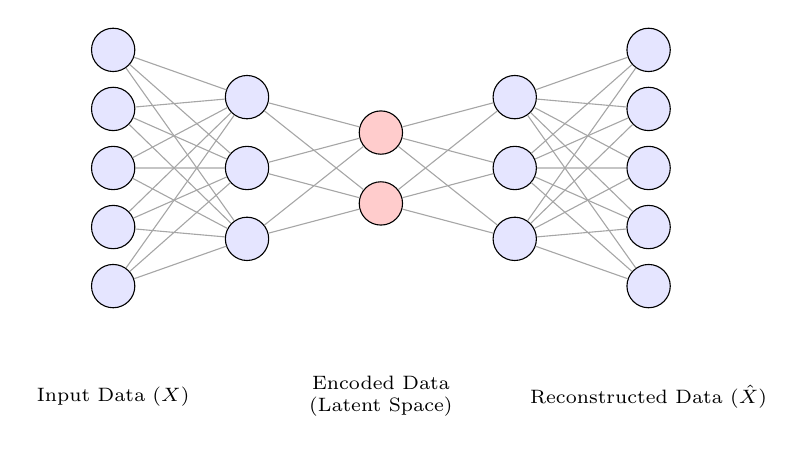
\begin{tikzpicture}[
    >=stealth,
    neuron/.style={
        circle,
        draw,
        minimum size=0.55cm,
        inner sep=0pt,
        fill=blue!10
    },
    bottleneck/.style={
        circle,
        draw,
        minimum size=0.55cm,
        inner sep=0pt,
        fill=red!20
    }
]

    % Input Layer
    \foreach \y in {1,2,3,4,5}
        \node[neuron] (I\y) at (0,\y*0.75-2.25) {};

    % Encoder Layer
    \foreach \y in {1,2,3}
        \node[neuron] (H1\y) at (1.7,\y*0.9-1.8) {};

    % Bottleneck Layer
    \foreach \y in {1,2}
        \node[bottleneck] (B\y) at (3.4,\y*0.9-1.35) {};

    % Decoder Layer
    \foreach \y in {1,2,3}
        \node[neuron] (H2\y) at (5.1,\y*0.9-1.8) {};

    % Output Layer
    \foreach \y in {1,2,3,4,5}
        \node[neuron] (O\y) at (6.8,\y*0.75-2.25) {};

    % Connections
    \foreach \i in {1,...,5}
        \foreach \j in {1,...,3}
            \draw[gray!70] (I\i) -- (H1\j);

    \foreach \i in {1,...,3}
        \foreach \j in {1,...,2}
            \draw[gray!70] (H1\i) -- (B\j);

    \foreach \i in {1,...,2}
        \foreach \j in {1,...,3}
            \draw[gray!70] (B\i) -- (H2\j);

    \foreach \i in {1,...,3}
        \foreach \j in {1,...,5}
            \draw[gray!70] (H2\i) -- (O\j);

    % Labels
    \node[font=\scriptsize] at (0,-2.9)
        {Input Data ($X$)};

    \node[font=\scriptsize, align=center] at (3.4,-2.9)
        {Encoded Data\\(Latent Space)};

    \node[font=\scriptsize] at (6.8,-2.9)
        {Reconstructed Data ($\hat{X}$)};

\end{tikzpicture}
}

\caption{Deep JSCC Autoencoder Architecture compressing and reconstructing data over a channel.}
\label{fig:autoencoder}

\end{figure}

The mathematical pipeline of the autoencoder is defined as follows:
\begin{enumerate}
    \item \textbf{Encoder Neural Network:} Maps the source data into channel symbols:
    \begin{equation}
        Z = f_\theta(X)
    \end{equation}
    \item \textbf{Channel Layer:} Introduces physical distortion and noise:
    \begin{equation}
        Y = H(Z)
    \end{equation}
    \item \textbf{Decoder Neural Network:} Reconstructs the data from the noisy received signal:
    \begin{equation}
        \hat{X} = g_\phi(Y)
    \end{equation}
\end{enumerate}
The entire communication pipeline can therefore be expressed as a single nested function:
\begin{equation}
    \hat{X} = g_\phi\Big(H(f_\theta(X))\Big)
\end{equation}

\subsection{\textbf{Channel Modeling as a Neural Layer}}
To enable end-to-end learning, the physical communication channel is inserted directly into the neural network during training as a non-trainable parameter layer. 

\begin{figure}[h]
\centering
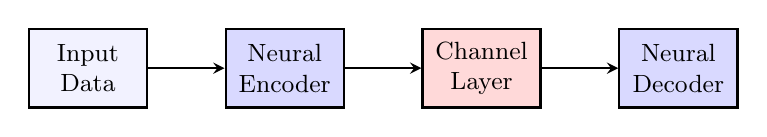
\begin{tikzpicture}[
    >=stealth,
    block/.style={draw, rectangle, fill=blue!5, minimum height=1cm, minimum width=1.5cm, align=center, font=\small, thick}
]
    \node[block] (in) at (0,0) {Input\\Data};
    \node[block, fill=blue!15] (enc) at (2.5,0) {Neural\\Encoder};
    \node[block, fill=red!15] (ch) at (5,0) {Channel\\Layer};
    \node[block, fill=blue!15] (dec) at (7.5,0) {Neural\\Decoder};
    

    \draw[->, thick] (in) -- (enc);
    \draw[->, thick] (enc) -- (ch);
    \draw[->, thick] (ch) -- (dec);
    
\end{tikzpicture}
\caption{Block Diagram of the Deep Learning Based JSCC Pipeline.}
\label{fig:jscc_pipeline}
\end{figure}

Two primary channel models are integrated into the network:
\subsubsection{AWGN Channel Layer}
The Additive White Gaussian Noise (AWGN) layer models thermal noise at the receiver. The decoder learns to mathematically compensate for this distribution:
\begin{equation}
    Y = X + N \quad \text{where} \quad N \sim \mathcal{N}(0, \sigma^2)
\end{equation}

\subsubsection{Rayleigh Fading Layer}
To simulate multi-path propagation environments, a Rayleigh fading coefficient ($h$) is introduced:
\begin{equation}
    Y = hX + N
\end{equation}
The neural network experiences fading during the training process, thereby autonomously learning robust transmission strategies without explicit pilot signals.

\begin{figure*}[t]
\centering
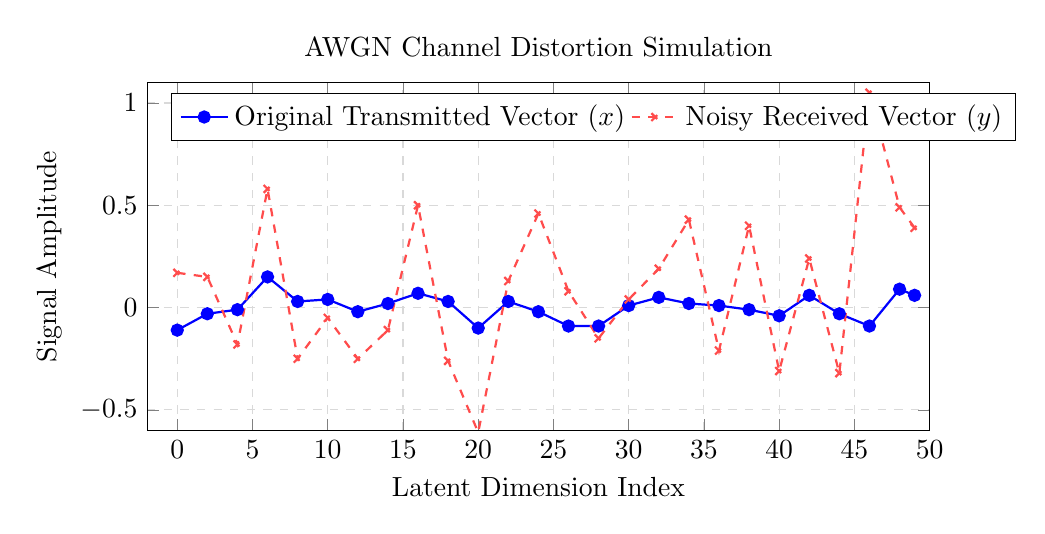
\begin{tikzpicture}
\begin{axis}[
    width=0.95\textwidth, height=6cm,
    xlabel={Latent Dimension Index}, ylabel={Signal Amplitude},
    title={AWGN Channel Distortion Simulation},
    legend pos=north west, legend columns=2,
    grid=both, grid style={dashed, gray!30},
    ymin=-0.6, ymax=1.1, xmin=-2, xmax=50
]
% Plotting synthetic representative data matching the visual graph provided
\addplot[blue, thick, mark=*, mark options={fill=blue}] coordinates {
    (0,-0.11) (2,-0.03) (4,-0.01) (6,0.15) (8,0.03) (10,0.04) (12,-0.02) 
    (14,0.02) (16,0.07) (18,0.03) (20,-0.10) (22,0.03) (24,-0.02) (26,-0.09) 
    (28,-0.09) (30,0.01) (32,0.05) (34,0.02) (36,0.01) (38,-0.01) (40,-0.04) 
    (42,0.06) (44,-0.03) (46,-0.09) (48,0.09) (49,0.06)
};
\addplot[red!70, thick, dashed, mark=x, mark options={fill=red}] coordinates {
    (0,0.17) (2,0.15) (4,-0.18) (6,0.58) (8,-0.25) (10,-0.05) (12,-0.25) 
    (14,-0.11) (16,0.50) (18,-0.26) (20,-0.61) (22,0.13) (24,0.46) (26,0.08) 
    (28,-0.15) (30,0.04) (32,0.19) (34,0.43) (36,-0.21) (38,0.40) (40,-0.31) 
    (42,0.24) (44,-0.32) (46,1.05) (48,0.49) (49,0.39)
};
\legend{Original Transmitted Vector ($x$), Noisy Received Vector ($y$)}
\end{axis}
\end{tikzpicture}
\caption{Visualization of original latent embeddings versus heavily distorted signals passing through an AWGN layer.}
\label{fig:awgn_noise}
\end{figure*}

\subsection{\textbf{Power Constraint Normalization}}
To ensure the transmitter emits finite energy over the physical channel, the encoder outputs ($Z$) are explicitly normalized. For an available transmit power $P$ and sequence length $k$, the constraint is bounded by:
\begin{equation}
    \frac{1}{k} \sum_{i=1}^{k} z_i^2 \leq P
\end{equation}
This is enforced dynamically within the network layers via the following transformation:
\begin{equation}
    Z = \sqrt{kP} \frac{Z}{||Z||}
\end{equation}

\subsection{\textbf{Optimization and Backpropagation}}
A fundamental advantage of Deep JSCC is the presence of a single loss function and a unified optimization process. The global loss function propagates backward from the receiver to the transmitter through the differentiable channel layer.
\begin{equation}
    \text{Goal:} \quad \min_{\theta, \phi} L(X, \hat{X})
\end{equation}
During backpropagation:
\begin{itemize}
    \item $\frac{\partial L}{\partial \phi}$ updates the receiver (decoder) parameters.
    \item $\frac{\partial L}{\partial \theta}$ updates the transmitter (encoder) parameters.
\end{itemize}

The loss configuration depends on the datatype being transmitted:
\begin{itemize}
    \item \textbf{For Images:} Mean Squared Error (MSE) is utilized.
    \begin{equation}
        L = \frac{1}{N} \sum_{i=1}^N (X_i - \hat{X}_i)^2
    \end{equation}
    \item \textbf{For Text:} Cross-Entropy Loss evaluates character/token probabilities.
    \begin{equation}
        L = - \sum y_i \log(\hat{y}_i)
    \end{equation}
\end{itemize}

\subsection{\textbf{Quality vs. Channel Degradation (The Cliff Effect)}}
Traditional communication protocols suffer from the "Cliff Effect". If the SNR falls below a specific threshold ($T$), the forward error correction fails completely, resulting in a sudden collapse of communication quality. 

Deep JSCC naturally avoids this. Since the quality is a direct learned function of SNR ($Quality = f(SNR)$), signal degradation is graceful and smooth, making it vastly superior for volatile wireless environments.

\begin{figure}[h]
\centering
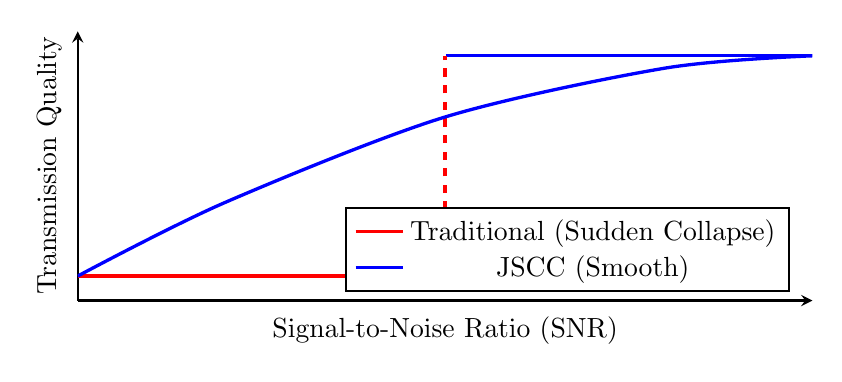
\begin{tikzpicture}
\begin{axis}[
    width=0.9\columnwidth, height=5cm,
    xlabel={Signal-to-Noise Ratio (SNR)}, ylabel={Transmission Quality},
    xmin=0, xmax=10, ymin=0, ymax=1.1,
    xtick=\empty, ytick=\empty,
    legend pos=south east,
    axis lines=left, thick
]
% Traditional Communication (Cliff Effect)
\addplot[red, very thick, domain=0:5] {0.1};
\addplot[blue, very thick, domain=5.01:10] {1.0};
\draw[red, very thick, dashed] (5,0.1) -- (5,1.0);

% JSCC Communication (Graceful Degradation)
\addplot[blue, very thick, smooth] coordinates {(0,0.1) (2,0.4) (5,0.75) (8,0.95) (10,1.0)};

\legend{Traditional (Sudden Collapse), JSCC (Smooth)}
\end{axis}
\end{tikzpicture}
\caption{Comparison of signal recovery quality: The traditional Cliff Effect versus the graceful degradation of JSCC.}
\label{fig:cliff_effect}
\end{figure}

\subsection{\textbf{JSCC for Semantic Communication}}
When extended into semantic communication, the Deep JSCC architecture is enveloped by Large Language Models (LLMs) or Transformer blocks to process intent rather than structural data. 

The loss function transitions from pixel/bit accuracy to Semantic Cosine Similarity, measuring the multi-dimensional angle between the original thought embedding ($E_X$) and the recovered meaning embedding ($E_{\hat{X}}$):
\begin{equation}
    L_{sem} = 1 - \frac{E_X \cdot E_{\hat{X}}}{||E_X|| ||E_{\hat{X}}||}
\end{equation}

\begin{figure}[h]
\centering
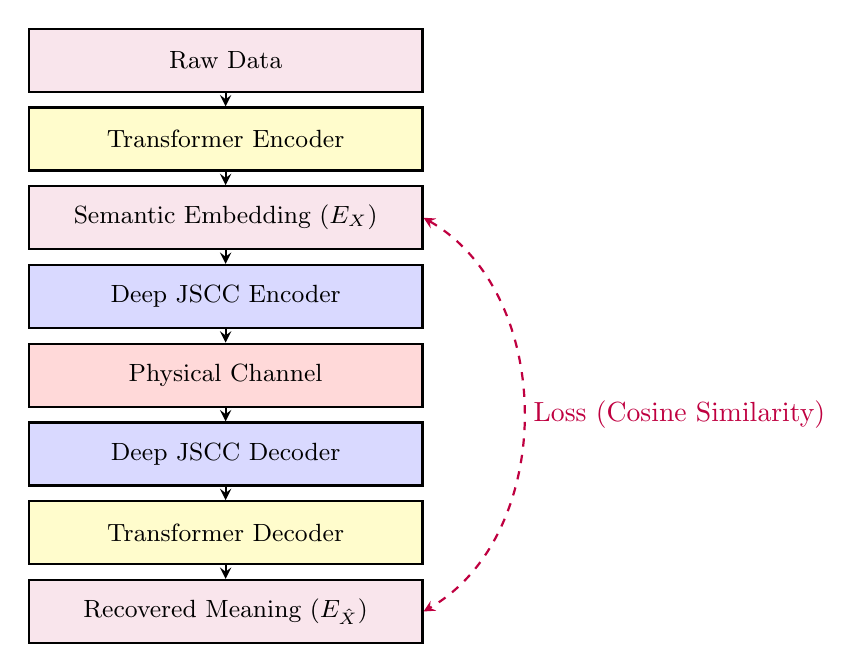
\begin{tikzpicture}[
    >=stealth,
    block/.style={draw, rectangle, fill=purple!10, minimum height=0.8cm, minimum width=5cm, align=center, font=\small, thick}
]
    \node[block] (raw) at (0,0) {Raw Data};
    \node[block, fill=yellow!20] (te) at (0,-1) {Transformer Encoder};
    \node[block] (se) at (0,-2) {Semantic Embedding ($E_X$)};
    \node[block, fill=blue!15] (jscc_e) at (0,-3) {Deep JSCC Encoder};
    \node[block, fill=red!15] (ch) at (0,-4) {Physical Channel};
    \node[block, fill=blue!15] (jscc_d) at (0,-5) {Deep JSCC Decoder};
    \node[block, fill=yellow!20] (td) at (0,-6) {Transformer Decoder};
    \node[block] (rec) at (0,-7) {Recovered Meaning ($E_{\hat{X}}$)};

    \draw[->, thick] (raw) -- (te);
    \draw[->, thick] (te) -- (se);
    \draw[->, thick] (se) -- (jscc_e);
    \draw[->, thick] (jscc_e) -- (ch);
    \draw[->, thick] (ch) -- (jscc_d);
    \draw[->, thick] (jscc_d) -- (td);
    \draw[->, thick] (td) -- (rec);
    
    % Loss indicator
    \draw[<->, dashed, thick, purple] (se.east) to[bend left=60] node[midway, right] {Loss (Cosine Similarity)} (rec.east);

\end{tikzpicture}
\caption{End-to-End Pipeline of JSCC optimized for Semantic Communication.}
\label{fig:semantic_jscc}
\end{figure}
\section{\large \textbf{Syntactic Drop and Information Bottleneck}}

\subsection{\textbf{Information Bottleneck Theory}}
The Information Bottleneck theory states that as a sentence gets longer, the fixed-size embedding vector doesn't have enough space to store every syntactic detail. Consequently, it drops the syntactic structure and preserves the semantic structure.

\subsection{\textbf{True Bottleneck Models vs. Matrix Output Models}}
In a true bottleneck model—which extracts only the CLS token or uses a fixed-size seq2seq bottleneck—the opposite behavior occurs. Both a small sentence and a large sentence would be compressed to the same $n$-dimensional vector. In this case, a long sentence would collapse much faster because its mathematical space is more crowded and highly sensitive to noise.

Conversely, a long sentence actually survives better than a short sentence in models like BART, which outputs a matrix of vectors (one vector for every single word). If noise destroys one word's vector, BART uses the other 19 words to guess the missing word. The short sentence simply didn't have enough surrounding context.

\begin{figure}[H]
\centering
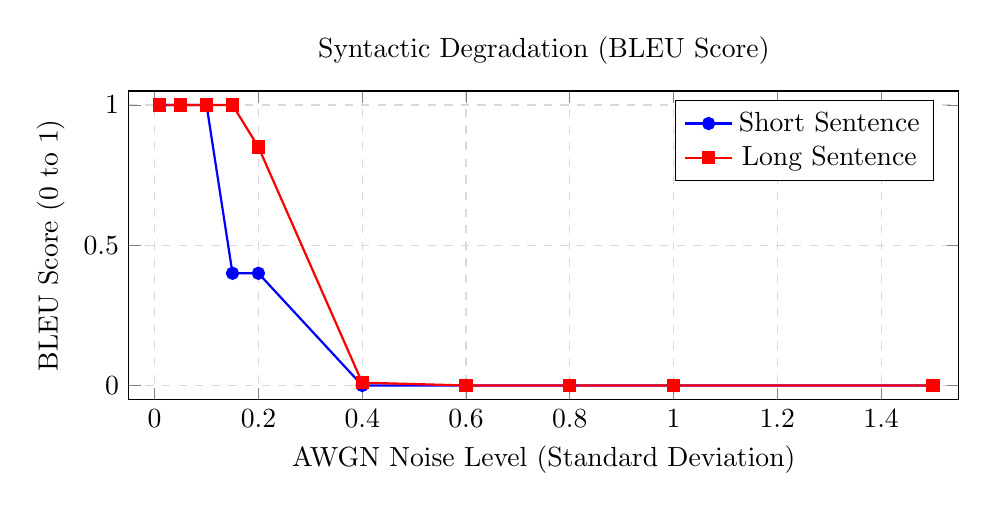
\begin{tikzpicture}
\begin{axis}[
    width=\columnwidth,
    height=5.5cm,
    title={Syntactic Degradation (BLEU Score)},
    xlabel={AWGN Noise Level (Standard Deviation)},
    ylabel={BLEU Score (0 to 1)},
    xmin=-0.05, xmax=1.55,
    ymin=-0.05, ymax=1.05,
    grid=both,
    grid style={dashed, gray!30},
    legend pos=north east
]
\addplot[color=blue, mark=*, thick] coordinates {
    (0.01,1) (0.05,1) (0.1,1) (0.15,0.4) (0.2,0.4) (0.4,0) (0.6,0) (0.8,0) (1.0,0) (1.5,0)
};
\addlegendentry{Short Sentence}
\addplot[color=red, mark=square*, thick] coordinates {
    (0.01,1) (0.05,1) (0.1,1) (0.15,1) (0.2,0.85) (0.4,0.01) (0.6,0) (0.8,0) (1.0,0) (1.5,0)
};
\addlegendentry{Long Sentence}
\end{axis}
\end{tikzpicture}

\vspace{0.5cm}

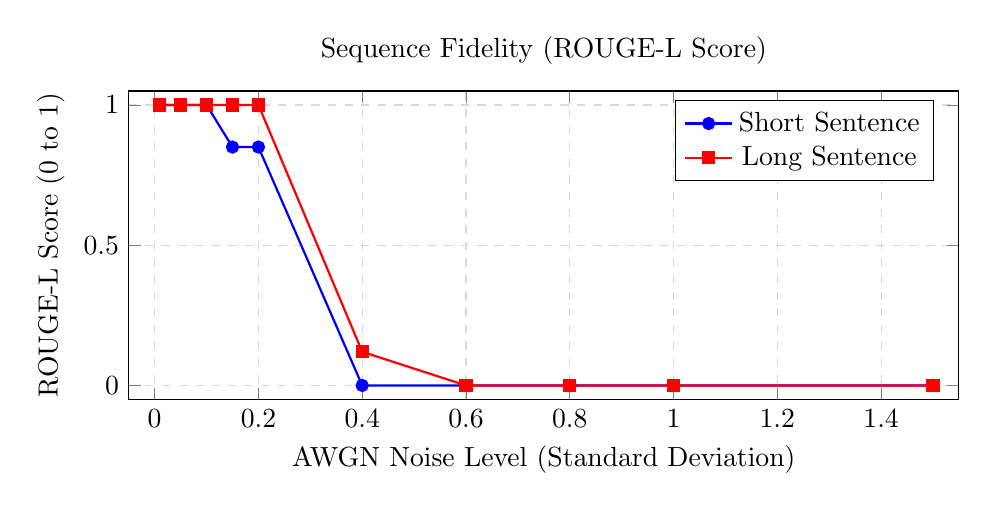
\begin{tikzpicture}
\begin{axis}[
    width=\columnwidth,
    height=5.5cm,
    title={Sequence Fidelity (ROUGE-L Score)},
    xlabel={AWGN Noise Level (Standard Deviation)},
    ylabel={ROUGE-L Score (0 to 1)},
    xmin=-0.05, xmax=1.55,
    ymin=-0.05, ymax=1.05,
    grid=both,
    grid style={dashed, gray!30},
    legend pos=north east
]
\addplot[color=blue, mark=*, thick] coordinates {
    (0.01,1) (0.05,1) (0.1,1) (0.15,0.85) (0.2,0.85) (0.4,0) (0.6,0) (0.8,0) (1.0,0) (1.5,0)
};
\addlegendentry{Short Sentence}
\addplot[color=red, mark=square*, thick] coordinates {
    (0.01,1) (0.05,1) (0.1,1) (0.15,1) (0.2,1) (0.4,0.12) (0.6,0) (0.8,0) (1.0,0) (1.5,0)
};
\addlegendentry{Long Sentence}
\end{axis}
\end{tikzpicture}
\caption{Impact of AWGN Noise Level on Syntactic Degradation and Sequence Fidelity for short vs. long sentences.}
\label{fig:noise_degradation}
\end{figure}


\section{\large \textbf{Sequence-to-Sequence (Seq2Seq) Models}}
Architectures such as T5 (Text-to-Text Transfer Transformer) and BART (Bidirectional and Auto-Regressive Transformer) are seq-seq models highly suitable for semantic extraction, semantic reconstruction, text compression, translation, etc. For a given input $X = (x_1, x_2, \dots, x_n)$, the model learns the distribution $P(Y|X)$.

\subsection{\textbf{T5 Architecture and Tokenization}}
T5 uses a full transformer encoder-decoder configuration. The T5 Tokenizer utilizes SentencePiece tokenization, which breaks words into subwords. For a text string $T$, the sequence is represented as:
\begin{equation}
    f(T) = [t_1, t_2, \dots, t_n]
\end{equation}
Each token $t_i$ is mapped to an integer ID, from which an embedding vector is derived:
\begin{equation}
    e_i = \text{Embedding}(t_i), \quad e_i \in \mathbb{R}^d
\end{equation}

\begin{figure}[H]
\centering
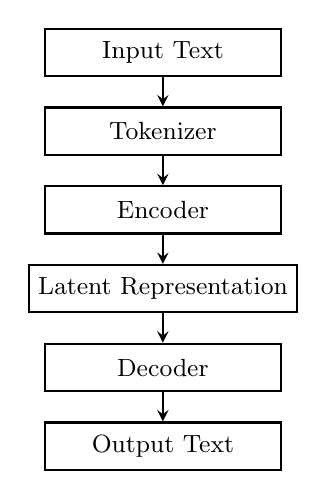
\begin{tikzpicture}[
    >=stealth,
    block/.style={draw, rectangle, minimum height=0.6cm, minimum width=3cm, align=center, font=\small, thick}
]
    \node[block] (ip) at (0,0) {Input Text};
    \node[block] (tok) at (0,-1.0) {Tokenizer};
    \node[block] (enc) at (0,-2.0) {Encoder};
    \node[block] (lat) at (0,-3.0) {Latent Representation};
    \node[block] (dec) at (0,-4.0) {Decoder};
    \node[block] (op) at (0,-5.0) {Output Text};

    \draw[->, thick] (ip) -- (tok);
    \draw[->, thick] (tok) -- (enc);
    \draw[->, thick] (enc) -- (lat);
    \draw[->, thick] (lat) -- (dec);
    \draw[->, thick] (dec) -- (op);
\end{tikzpicture}
\caption{Structural flow of the T5 Architecture.}
\label{fig:t5_arch}
\end{figure}

Each encoder layer computes the sequence iteratively:
\begin{equation}
    H^{(l)} = \text{FFN}\big(\text{attention}(H^{(l-1)})\big)
\end{equation}
After processing through multiple layers, the final state array $H = [h_1, h_2, \dots, h_n]$ contains the consolidated semantic information.

\subsection{\textbf{T5 Decoder and Span Corruption}}
The T5 decoder generates the output autoregressively at step $t$:
\begin{equation}
    P(y_t \mid y_{<t}, H)
\end{equation}
Meaning, the current token strictly depends on:
\begin{itemize}
    \item Previously generated tokens ($y_{<t}$)
    \item Encoder semantic information ($H$)
\end{itemize}
The overall sequence generation probability follows:
\begin{equation}
    P(Y|X) = \prod_{t=1}^{m} P(y_t \mid y_{<t}, X)
\end{equation}
Instead of predicting the next word natively, T5 performs \textbf{Span Corruption}: the model learns from corrupted text to deduce missing text. This mechanism forcefully instills deep semantic understanding.


\section{\large \textbf{BART Architecture and Role in Communication}}
To contextualize the evolutionary mapping of transformer models:
\begin{itemize}
    \item \textbf{BERT:} Encoder only
    \item \textbf{GPT:} Decoder only
    \item \textbf{BART:} Encoder + Decoder
\end{itemize}

\subsection{\textbf{BART Corruption Process}}
The fundamental BART architecture routes from the input $[i/p]$ into a $[transformer\ encoder]$ block to extract a $[latent\ representation]$, which is then parsed by the $[transformer\ decoder]$ to yield the $[o/p]$. The defining noise-corruption and training pipeline is:
\begin{itemize}
    \item Original data: $X$
    \item Noise function: $\tilde{X} = N(X)$
    \item Encoder processes: $\tilde{X}$
    \item Decoder reconstructs: $\hat{X}$
    \item Training objective: $\min \rightarrow \log_P(X \mid \tilde{X})$
\end{itemize}

\subsection{\textbf{Role in Semantic Communication}}
In a functional physical layer, these NLP architectures operate as Joint Source-Channel Coding (JSCC) entities. 

\section{\large \textbf{Tokenization Theory}}

Before compressing a sentence into a mathematical vector, we must convert the raw text into discrete integers that the neural network can process. This foundational process is called \textbf{Tokenization}. 

Neural networks cannot read strings directly. Therefore, we must scan the dataset, build a comprehensive lookup table, and map every unique word to a unique integer representation.

\begin{table}[htbp]
\centering
\caption{Example of a Tokenization Lookup Table}
\label{tab:lookup_table}
\begin{tabular}{ccc}
\toprule
\textbf{Word (String)} & & \textbf{Integer ID} \\
\midrule
Arpit & $\rightarrow$ & 4312 \\
School & $\rightarrow$ & 1284 \\
Rescue & $\rightarrow$ & 1001 \\
VLSI & $\rightarrow$ & 724 \\
Aadya & $\rightarrow$ & 9901 \\
AI & $\rightarrow$ & 1234 \\
\bottomrule
\end{tabular}
\end{table}

To train a robust model over a noisy communication channel, we must define 4 specialized tokens to handle structural variations and sequence control:

\subsection{\textbf{1. \textless PAD\textgreater \ (ID: 0)}}
If sentence A has 5 words and sentence B has 10 words, we must append 5 \texttt{\textless PAD\textgreater} tokens to sentence A so that both sequences possess exactly 10 words. This standardisation is strictly necessary as neural networks process data in parallel batches and require uniform matrix dimensions.

\subsection{\textbf{2. \textless UNK\textgreater \ (ID: 1)}}
When encountering a word that has never been seen before in the training dataset, the model replaces it with the \texttt{\textless UNK\textgreater} (Unknown) token. This forces the Long Short-Term Memory (LSTM) network or Transformer to rely entirely on the surrounding context to guess the meaning of the unknown word.

\subsection{\textbf{3. \textless BOS\textgreater \ (ID: 2)}}
When an LSTM decoder wants to reconstruct a sentence from a noisy semantic vector, it needs a definitive trigger to know it is time to generate the very first word. To initiate this generation sequence, we feed it the \texttt{\textless BOS\textgreater} (Beginning of Sentence) token.

\subsection{\textbf{4. \textless EOS\textgreater \ (ID: 3)}}
If the \texttt{\textless EOS\textgreater} (End of Sentence) token is not present, the decoder will theoretically keep predicting words forever. Once the \texttt{\textless EOS\textgreater} token is predicted, the receiver network definitively knows the sequence transmission is complete.


\section{\large \textbf{Tokenization \& Mathematics}}

\subsection{\textbf{Zipf's Law \& The \textless UNK\textgreater \ Danger Zone}}
In linguistics and information theory, the semantic information carried by a word is inversely proportional to its frequency of occurrence. Mathematically, the information content $I(x)$ of a symbol $x$ is defined as:
\begin{equation}
    I(x) = -\log P(x)
\end{equation}

Words like "the", "a", or "is" carry almost no significant semantic meaning, but they occur a massive number of times within a dataset. Conversely, highly specific words occur rarely but carry the bulk of the sentence's meaning.

\begin{figure}[htbp]
\centering
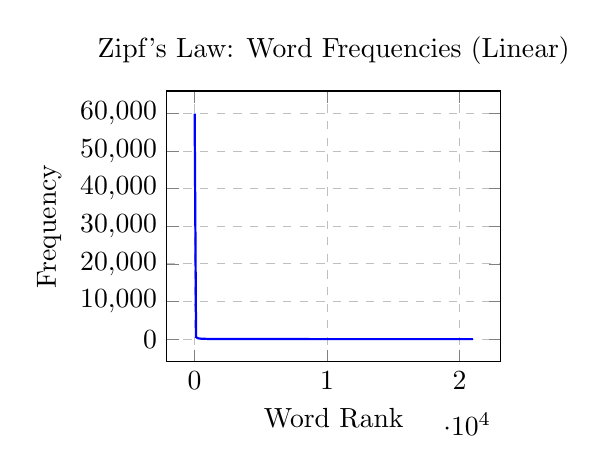
\begin{tikzpicture}
\begin{axis}[
    width=0.48\textwidth, title={Zipf's Law: Word Frequencies (Linear)},
    xlabel={Word Rank}, ylabel={Frequency}, grid=both, grid style=dashed,
    scaled y ticks=false, ytick={0, 10000, 20000, 30000, 40000, 50000, 60000}
]
\addplot[blue, thick, domain=1:21000, samples=200] {60000/x};
\end{axis}
\end{tikzpicture}
\hfill
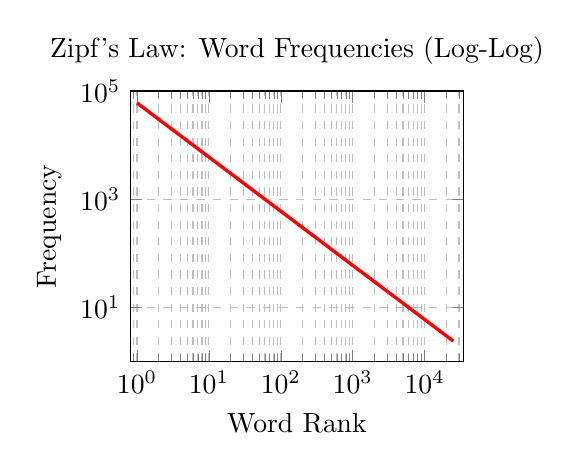
\begin{tikzpicture}
\begin{axis}[
    width=0.48\textwidth, title={Zipf's Law: Word Frequencies (Log-Log)},
    xmode=log, ymode=log, xlabel={Word Rank}, ylabel={Frequency}, 
    grid=both, grid style=dashed,
    ymin=1, ymax=100000, xmin=0.8, xmax=35000
]
\addplot[red, very thick, domain=1:25000, samples=100] {60000/x};
\end{axis}
\end{tikzpicture}
\caption{Visual demonstration of Zipf's Law showing the inverse relationship between word rank and frequency across linear and log-log scales.}
\label{fig:zipfs_law}
\end{figure}

When creating the vocabulary lookup table, setting a minimum frequency threshold filters out rare words (replacing them with \texttt{\textless UNK\textgreater}) to save memory. However, if you keep the minimum frequency threshold too high, the majority of the true data volume and semantic meaning is destroyed.

\begin{figure}[htbp]
\centering
\begin{tikzpicture}
\begin{axis}[
    ybar, width=0.9\columnwidth, height=6.5cm,
    title={Semantic Volume Loss},
    xlabel={Threshold (Minimum Frequency)}, 
    ylabel={\% of words Replaced by \textless UNK\textgreater},
    symbolic x coords={1, 2, 5, 10, 50, 100},
    xtick=data,
    nodes near coords={\pgfmathprintnumber\pgfplotspointmeta\%}, 
    nodes near coords align={vertical},
    every node near coord/.append style={font=\bfseries},
    grid=y, grid style=dashed,
    ymin=0, ymax=20, bar width=25pt
]
\addplot[fill=orange, draw=black, thick] coordinates {
    (1,0.0) (2,1.0) (5,2.6) (10,4.4) (50,12.1) (100,18.1)
};
\end{axis}
\end{tikzpicture}
\caption{Dependence of semantic volume loss on the minimum frequency threshold. A higher threshold heavily degrades the underlying meaning of the dataset.}
\label{fig:semantic_volume_loss}
\end{figure}

\subsection{\textbf{The Padding Tax}}
While padding is necessary for matrix operations, transmitting a \texttt{\textless PAD\textgreater} token through a physical 6G channel consumes actual electrical power and physical bandwidth for absolutely zero semantic gain. This phenomenon is referred to as the \textbf{padding tax}.

\begin{figure}[htbp]
\centering
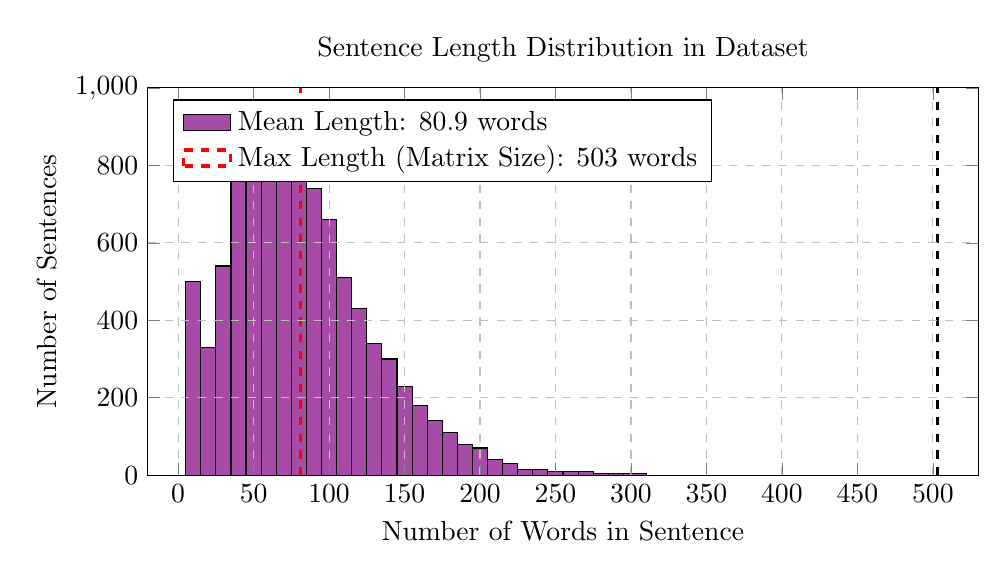
\begin{tikzpicture}
\begin{axis}[
    width=\columnwidth, height=6.5cm,
    title={Sentence Length Distribution in Dataset},
    xlabel={Number of Words in Sentence}, 
    ylabel={Number of Sentences},
    grid=both, grid style=dashed,
    xmin=-20, xmax=530, ymin=0, ymax=1000,
    area style,
    legend cell align={left},
    legend pos=north west
]
% Approximation of the provided right-skewed histogram
\addplot+[ybar interval, fill=violet!70, draw=black, mark=none] coordinates {
    (5, 500) (15, 330) (25, 540) (35, 810) (45, 920) (55, 880) (65, 920) 
    (75, 840) (85, 740) (95, 660) (105, 510) (115, 430) (125, 340) (135, 300) 
    (145, 230) (155, 180) (165, 140) (175, 110) (185, 80) (195, 70) (205, 40)
    (215, 30) (225, 15) (235, 15) (245, 10) (255, 10) (265, 10) (275, 5) 
    (285, 5) (295, 5) (310, 0)
};

\addplot[red, dashed, very thick] coordinates {(80.9,0) (80.9,1000)};
\addlegendentry{Mean Length: 80.9 words}

\addplot[black, dashed, very thick] coordinates {(503,0) (503,1000)};
\addlegendentry{Max Length (Matrix Size): 503 words}

\end{axis}
\end{tikzpicture}
\caption{Visualization of the padding tax. Because the matrix must accommodate the maximum length sequence (503 words), the vast majority of shorter sentences (mean 80.9) are heavily padded with useless zeros.}
\label{fig:padding_tax}
\end{figure}

Because the neural network input matrix must be sized to accommodate the absolute longest sentence in the dataset (e.g., 503 words), every shorter sentence (which averages around 80.9 words) must be artificially padded up to length 503, drastically inflating transmission overhead.


\subsection{\textbf{Shannon Entropy}}
Derived directly from the token probabilities, the Shannon Entropy establishes the theoretical lower bound of compression. It defines the absolute minimum average number of bits required to transmit a symbol:
\begin{equation}
    H = - \sum P(x) \log_2 P(x)
\end{equation}
In the context of semantic networks, entropy guides how densely we can pack our numerical vectors without violating the fundamental limits of information reconstruction at the receiver end.



\end{document}